%
%      File Name : thesis.tex
%  Creation Date : 07-08-2012
%  Last Modified : Tue Jan 29 15:48:33 2013
%

\documentclass[11pt,letterpaper,]{thesis2}
%%
% File - thesis_definitions.tex
%
%
% Description:
% This file should contain all the definitions used in your thesis.
%
% Examples:
% \def\dx\{d\!x}}
% \def\cD{\cal{D}} ... etc ...
%

%
% File thesis_environment.tex
%
% Description:
% This file contains environments for theorems, lemmas, definitions,
% proofs, corollaries, algorithms, examples, remarks, and assumptions.
% The numbering is set up so that the same counter is used for ALL
% these environments.  This seems to make it easier for readers to
% find referenced material.  The counter is reset for each chapter.
%
% EXAMPLE
%    Definition 3.1
%    Lemma 3.2
%    Example 3.3
%    Theorem 3.4
%    Theorem 3.5
%    Lemma 3.6 ....
%
%    Lemma 4.1
%    Corollary 4.2 ....
%
% The Definition environment is indented on both sides.  This
% is not required, but seemed to be a nice way to separate definitions
% from proven results.
%
\usepackage{graphicx}
\usepackage{floatrow}


\usepackage{listings}
\usepackage{color}

\definecolor{dkgreen}{rgb}{0,0.6,0}
\definecolor{gray}{rgb}{0.5,0.5,0.5}
\definecolor{mauve}{rgb}{0.58,0,0.82}

\lstset{frame=tb,
  language=C,
  %aboveskip=3mm,
  %belowskip=3mm,
  showstringspaces=false,
  columns=flexible,
  basicstyle={\small\ttfamily},
  numbers=none,
  numberstyle=\tiny\color{gray},
  keywordstyle=\color{blue},
  commentstyle=\color{dkgreen},
  stringstyle=\color{mauve},
  breaklines=true,
  breakatwhitespace=true,
  tabsize=3
}
%%%%%%%%%%%%%%%%%%%%%%%%%%%%%%%%%%%%
\newtheorem{thm}{Theorem}[chapter]
\newtheorem{lemma}[thm]{Lemma}
\newtheorem{cor}[thm]{Corollary}
\newtheorem{prop}[thm]{Proposition}
\newtheorem{defin}[thm]{Definition}
\newtheorem{obser}[thm]{Observation}
\newtheorem{remark}[thm]{Remark}
%%%%%%%%%%%%%%%%%%%%%%%%%%%%%%%%%%%%%%%%%%%%%%%%%%%%
\newenvironment{definition}{\begin{description}\begin{defin}}
{\end{defin}\end{description}\medskip}
\newenvironment{proof}{{\bf Proof:} }{\hfill\rule{2.1mm}{2.1mm}}
%%%%%%%%%%%%%%%%%%%%%%%%%%%%%%%%%%%%%%%%%%%%%%%%%%%%
\newfloatcommand{capbtabbox}{table}[][\FBwidth]
\floatsetup[table]{capposition=top}


\newcounter{example}
\newenvironment{example}{\refstepcounter{example}
         \medskip\par\noindent\textbf{Example \theexample.} } {\medskip}

\begin{document}

% Set page numbering -- ToDo
\pagenumbering{roman}
\pagestyle{empty}

%%%%%%%%%%%%%%%%%%%
% Title page
%%%%%%%%%%%%%%%%%%%
\title{POINT IN POLYGON (PIP) SEARCH ACCELERATION USING GPU BASED QUADTREE FRAMEWORK}
\author{SREEVIDDYADEVI}{KARUNAGARAN}
\otherdegrees{B.E., Anna University, India, 2008}
%\degree{Master of Science}{M.S., Applied Mathematics}
\degree{Master of Science}{M.S., Electrical Engineering}
\degreeyear{2016} \dept{Electrical Engineering}{}
\titlepage

\pagestyle{fancy}

%%%%%%%%%%%%%%%%%%%
% Approval Page
%  note: Ph.D. students may add more readers as needed.
%%%%%%%%%%%%%%%%%%%
\advisor{Professor}{Dan Connors}
\readerone{Dan Connors}
\readertwo{Yiming Deng}
\readerthree{Chao Liu}
\chair{Dan Connors}
\newdate{defensedate}{14}{04}{2016} % <day>, <month>, <year> 
\approvalpage

%%%%%%%%%%%%%%%%%%%
% Abstract Page -- ToDo
%%%%%%%%%%%%%%%%%%%
\abstractpage{%
% File - thesis_abstract.tex
%
%
% Description:
% Write your abstract in this file.
%
%
%
The point-in-polygon (PIP) problem defines for a given set of points
in a plane whether those points are inside, outside or on the
boundary of a polygon. The PIP for a plane is a special case of point
range finding that has applications in numerous areas that deal with
processing geometrical data, such as computer graphics, computer
vision, geographical information systems (GIS), motion planning and
CAD. Point in range search can be performed by a brute force search
method, however solution becomes increasingly prohibitive when
scaling the input to a large number of data points and distinct
ranges (polygons). The core issue of the brute force approach is that
each data point must be compared to the boundary range requiring
both computation and memory access.  By using a spatial data structure
such as a quadtree, the number of data points computationally compared
within a specific polygon range can be reduced to be more efficient in
terms of performance on the CPU.  While Graphics Processing Unit (GPU) 
systems have the potential to advance the computational requirements
of a number of problems, their massive number of processing cores
execute efficiently only in certain rigid execution models such as
data-level parallel problems. The goal of this thesis is to demonstrate
that the GPU systems can still process irregular data structure such
as a quadtree and that it can be efficiently traversed on a GPU to find the points
inside a polygon. Compared with an optimized serial CPU implementation
based on the recursive Depth-First Search (DFS), the stack based
iterative Breadth-first search (BFS) on the GPU has a performance gain
of 3x to 500x.
\newpage

}

%%%%%%%%%%%%%%%%%%%
% Dedication page
%%%%%%%%%%%%%%%%%%%
% \pagestyle{empty}
%\clearpage \vspace*{.25in}
%\centerheading{DEDICATION}
%\begin{block}
%%
% File - dedication.tex
%
%
% Description:
% Write you dedication in this file
%
This file is dedicated to Gary, my pet chimpanzee, who watched at
my side as I proved theorems and wrote my thesis.

%\end{block}
%\newpage

%%%%%%%%%%%%%%%%%%%
% Acknowledgment page
%%%%%%%%%%%%%%%%%%%
%\clearpage \vspace*{.25in}
%\centerheading{ACKNOWLEDGMENT}
%\begin{block}
%%
% File - thanks.tex
%
%
% Descrption:
% This file should contain any acknowledgment you would like to give.
% (Like your advisor for example.)
%
%
This thesis would not have been possible without the generous
support of Great Aunt Penelope.

%\end{block}
%\newpage

%%%%%%%%%%%%%%%%%%%
% Table of contents
%%%%%%%%%%%%%%%%%%%
% \pagestyle{plain}
\tableofcontents
\listoftables
\listoffigures

%%%%%%%%%%%%%%%%%%%%%
% Start first chapter
%%%%%%%%%%%%%%%%%%%%%
% reset page numbering -- ToDo
\setcounter{page}{0}
\pagenumbering{arabic}

\chapter{Introduction}\label{chap:Introduction}
%
% File - ch1.tex
%
%
% Description:
% This file should contain the first real chapter or section of your
% thesis.
%
%
% 1st paragraph is background on concept of computer vision
%Computer vision is what and why is it important....

The point-in-polygon (PIP) problem defines for a given set of points
in a plane whether those points are inside, outside or on the
boundary of a polygon. The PIP for a plane is a special case of point
range finding that has applications in numerous areas that deal with
processing geometrical data, such as computer graphics, computer
vision, geographical information systems (GIS), motion planning and
CAD. Point in range search can performed by a brute force
search method, however for solution becomes increasingly prohibitive
when scaling the input to a large number of data points and distinct
ranges (polygons).

Range search algorithms, which make use of spatial data structures,
perform much better than the ones that do not partition the data
before processing. Quadtree is a hierarchical spatial data structure
that is used for both indexing and compressing geographic database
layers due its applicability to many types of data, its ease of
implementation and relatively good performance. 
As done traditionally, the quadtree is built on the CPU. To speed up
the range searching problems, it is essential to increase the
threshold on the number of queries processed within a given time
frame. Purely sequential approach to this will demand increase in
processor speeds.  

Graphics Processing Units (GPUs) have proven to be
a powerful and efficient computational platform. An increasing number
of applications are demanding more efficient computing power at a
lower cost.  The modern GPU can natively perform thousands of parallel
computations per clock cycle.  Relative to the traditional power of a
CPU, the GPU can far out-perform the CPU in terms of computational
power or Floating Point Operations per Second (FLOPS). Traditionally
GPUs have been used exclusively for graphics processing. Recent
developments have allowed GPUs to be used for more than just graphics
processing and rendering. With a growing set of applications these
new GPUs are known as GPGPUs (General Purpose GPUs).
NVIDIA\textsuperscript{\textregistered} has developed the CUDA 
(Compute Unified Device Architecture) API (Application Programming
Interface) which enables software developers to access the GPU through
standard programming languages such as 'C'.  CUDA gives developers
access to the GPU's virtual instruction set, onboard memory and the
parallel computational elements.  Taking advantage of this parallel
computational power will result in significant speedup for multiple
applications.  One such application is computer vision algorithms.
From the assembly line to home entertainment systems, the need for
efficient real-time computer vision systems is growing quickly.  This
paper explores the potential power of using the CUDA API and
NVIDIA\textsuperscript{\textregistered} GPUs to speedup common
computer vision algorithms.  Through real-life algorithm optimization
and translation, several approaches to GPU optimization for existing
code are proposed in this report.

%% Premise : GPU doesn't hangle irregular
In the past few years, there has been a rapid adoption of GPGPU
parallel computing techniques for both high-performance computing and
mobile systems.  As GPUs exploit models of data-parallel execution
that generally describes a common task across different parallel
computing elements, there can be severe limitations for any irregular
individual thread behaviors.  Irregular execution disrupts the
efficiency of the rigid GPU groups of threads by causing workload
disparity that effectively leads to idle or underutilized resource
units.  Most research focus is on the hardware aspects of execution
disparity such as branch divergence~\cite{divergence1}, local memory
bank conflicts~\cite{local} and non-coalesced global memory
accesses~\cite{memory}.  There are a number of proposed architecture
concepts to mitigate some of the performance downfalls of handling
non-uniform data on GPU architectures~\cite{divergence2}.  Many of the
proposed solutions reduce the frequency of the occurrences but do not
fully address the inherent run-time execution characteristics of an
algorithm. Overall,
irregular data patterns limit the performance potential of GPGPU
algorithms.

%% There are attempts to solve the problem
While irregular algorithms restrain the full use of data-level
resources of GPU systems, GPU implementations may still achieve
performance benefit over multicore implementations. In effect, the raw
number of GPU resources serves as a brute-force method of carrying out
computations with significant arithmetic intensity.  Nevertheless,
there are alternative and emerging software-based models of
distributing execution tasks on GPUs such as dynamic parallelism
support. Another technique proposed is persistently scheduled thread
groups~\cite{Gupta:2012:ASO} that abandons the traditional data-level
model for stable thread groups assigned to GPU compute units that
dynamically retrieve computation tasks from software-based workload
queues.  The result of persistently scheduled groups can be better
load balance, utilization and reduced overhead in thread block
creation. At the same time, such techniques have not fully addressed
exploiting patterns and variations in model data specific to
algorithms.

%% What are the problems
Generally tasks that involve irregular data or non-deterministic
algorithms are not effectively mapped to GPU systems.  For example, in
graph-based algorithms, the irregular nature of the edge connectivity
between graph nodes is not well suited for data-level task definition
on GPU computing units. In this case, a group of neighboring GPU
threads may be assigned a diverse workload of processing nodes with a
few edges as well as nodes with thousands of edges.  This form of
imbalance is characterized as {\em static workload disparity} as a
portion of the runtime utilization can be traced to the static
connectivity of graph nodes.  Only if a graph's structure is
persistent, not changing over several evaluations, might there be
well-reasoned opportunities to reorganize the data, effectively
performing static load balancing in which each GPU thread group is
assigned data with less variation in work.  However, in such cases,
there is cost to the partitioning graph nodes to the model data.

This thesis investigates the potential of processing quadtrees for PIP search problems
that execute on GPUs.  As GPUs operate in a heterogeneous system in which both
the CPU and GPU perform some fraction of the computational work, there are
unique performance constraints to explore.  This thesis considers two primary parameters
in scaling optimal GPU quad-tree solutions: data point problem size and characteristics of polygons being searched.


This thesis is organized as follows:
Chapter~\ref{chap:background} discusses the motivation and background of computer vision applications.
Chapter~\ref{chap:approach} examines several examples of the PIP problem solving on GPUs.
The experimental results section, Chapter~\ref{chap:results}, shows performance
data for the various optimization cases.  Finally, Chapter~\ref{chap:conclusion} concludes this
thesis.


\chapter{Background and Motivation}\label{chap:background}
%
% File - ch1.tex
%
%
% Description:
% This file should contain the first real chapter or section of your
% thesis.
%
%
%%%%%%%%%%%%%%%%%%%%%%%%%%%%%%%%%%%%%%%%%%%%%%%%%%%%%%%%%%%%%%%%%%%%%%%%%%%%%%%
\section{Quadtree Background}~\label{sec:quadtree_motivation}
%%%%%%%%%%%%%%%%%%%%%%%%%%%%%%%%%%%%%%%%%%%%%%%%%%%%%%%%%%%%%%%%%%%%%%%%%%%%%%%

A quadtree is a tree data structure that designates each internal node
to have exactly 4 children. Quadtrees are used to partition a 2D space
by recursively subdividing it into 4 quadrants or regions. The regions
may be square or rectangular or may have arbitrary shapes. Quadtrees
may be classified according to the type of data represented such as
areas, points, lines and curves. Figure~\ref{fig:quadtree}
demonstrates a set of 2D data points that have been used to compose a
quadtree. The reasoning for using a quadtree structure is that any
region search that requires the data points within a polygon area
simply can reference the tree rather than the data.  There are clear
search benefits from the data to tree representations. In the case of
the lower right quadrant, any region search will consult the tree
structure and determine that only a limited number of point values 
(X, Y) are required for comparison.  In short, the tree representation
saves the computational calculations for the polygon search by
immediately directing that only a limited number of points exist in
that entire quadrant.  In the comparison case, it is easier for a
polygon that resides in the lower right quadrant to consult the tree
versus consult the full data set using full brute force checking of
every datapoint within the polygon range.

\begin{figure} [H]
    \begin{center}
    \vspace{0.5in}
    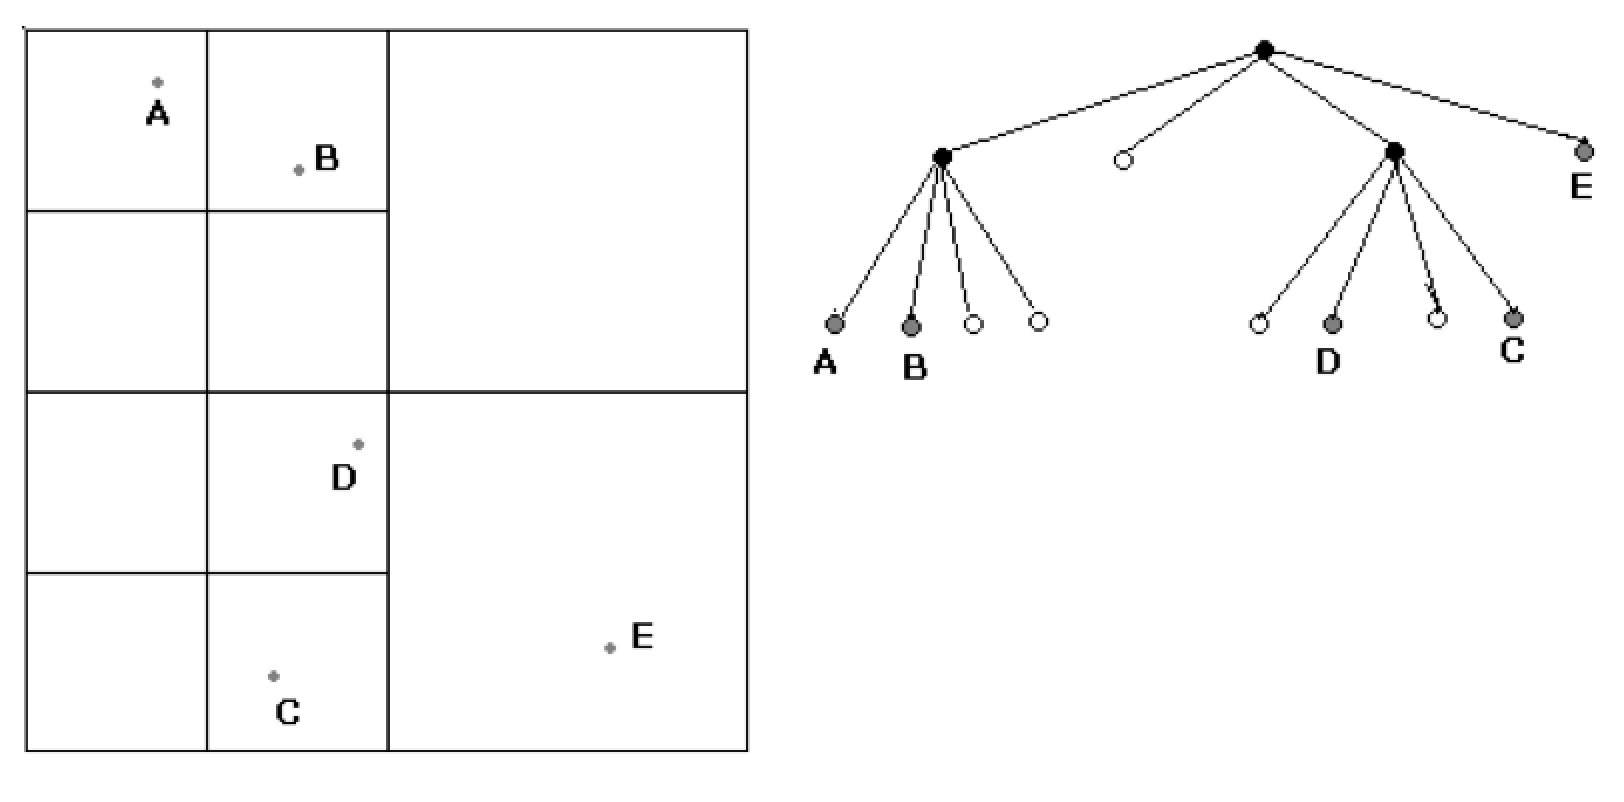
\includegraphics[scale=0.5]{Images/webQuad}
    \vspace{0.5in}
    \end{center}
    \caption{Example of Data Points Mapped within a Quadtree Data Structure.}
    \label{fig:quadtree}
\end{figure}



\subsection{Quadtree Construction}

Figure~\ref{fig:quadtree_construction1},
Figure~\ref{fig:quadtree_construction2},
Figure~\ref{fig:quadtree_construction3},
Figure~\ref{fig:quadtree_construction4}, demonstrates quadtree
construction on the CPU up to level 4.
The Figure~\ref{fig:quadtree_construction1}, shows the sample data points
at level 1 and it represents the root node containing all the data points.
The Figure~\ref{fig:quadtree_construction2}, shows the sample data points
at level 2 and it represents the four child nodes of the root node.
The Figure~\ref{fig:quadtree_construction2} is further subdivided to generate 
level 3 of the quadtree as shown in Figure~\ref{fig:quadtree_construction3}.
The Figure~\ref{fig:quadtree_construction4}, represents the tree at level 4.
There are two empty nodes at level 4, as there no points in that direction. 

 \begin{figure}[H]   
 \centering
 \vspace{0.5in}
 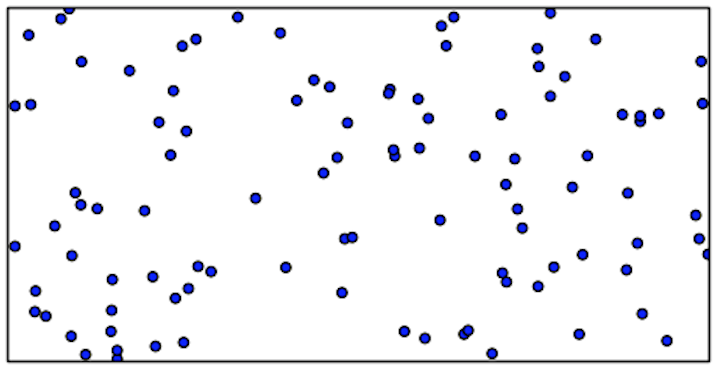
\includegraphics[scale=0.5]{Images/Quadtree_construction1}
 \vspace{0.5in}
 \caption{Level 1 of Quadtree.}
 \label{fig:quadtree_construction1}
 \end{figure}


 \begin{figure}[H]
 \centering
 \vspace{0.5in}
 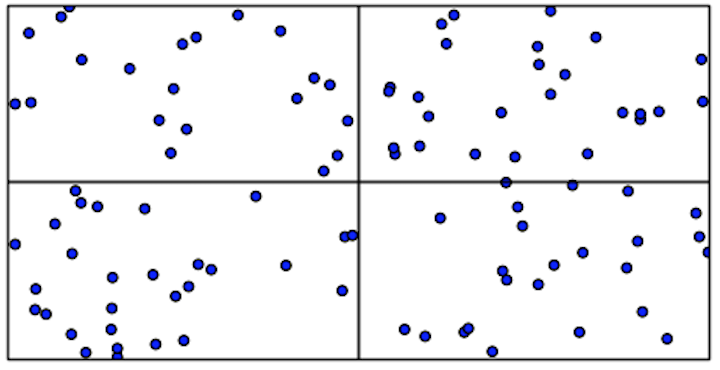
\includegraphics[scale=0.5]{Images/Quadtree_construction2}
 \vspace{0.5in}
 \caption{Level 2 of Quadtree.}
 \label{fig:quadtree_construction2}
 \end{figure}  

  \begin{figure}[H]    
  \centering
  \vspace{0.5in}
  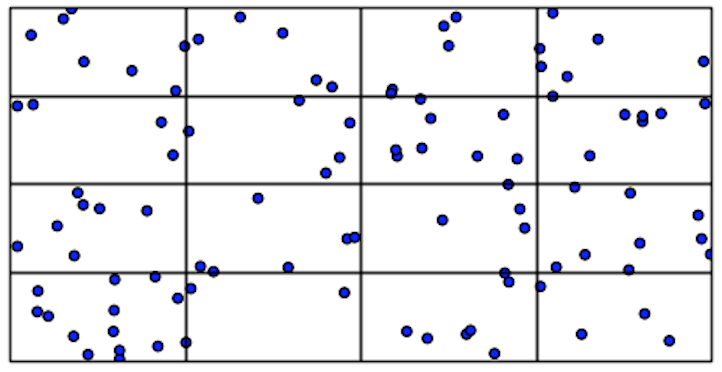
\includegraphics[scale=0.5]{Images/Quadtree_construction3}
  \vspace{0.5in}
  \caption{Level 3 of Quadtree.}
  \label{fig:quadtree_construction3} 
  \end{figure}

 \begin{figure}[H]    
 \centering
 \vspace{0.5in}
 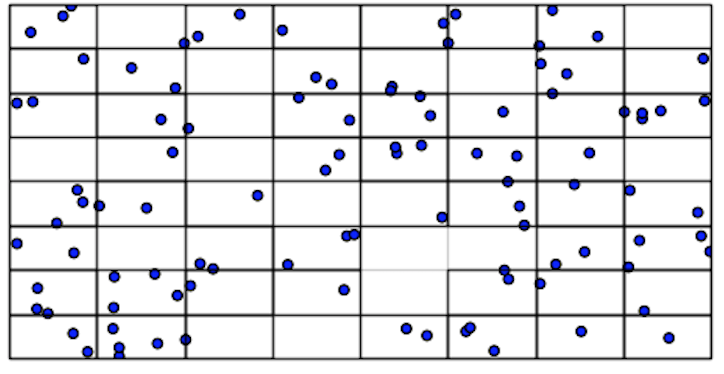
\includegraphics[scale=0.5]{Images/Quadtree_construction4}
 \vspace{0.5in}
 \caption{Level 4 of Quadtree.}
 \label{fig:quadtree_construction4}
 \end{figure}


The point quadtree structure recursively divides space into four equal 
rectangles based on the location of the points. The root of the quadtree 
represents the whole 2D space. Successive points divide each 
new sub-region into quadrants until all points are indexed. With each 
subsequent level, quadtrees can have a maximum of four children for 
every parent node. Each node represents a region in the 2D space
which contains a subset of the data points.

The common algorithm to construct a quadtree is based on sequential
 point insertion and this sequential approach is not suitable for
 massively parallel processors. Therefore the quadtree construction is
 done on the CPU. The performance of quadtrees, for Insertion is O(n
 log n), for searching is O(log n) and optimization for the purposes
 of balancing the tree is O(n log n) \cite{Kelly:gpu}. This makes quadtrees an ideal data
 structure for multiple insertion of points and range searching \cite{Kelly:gpu}.
 Though the linear quadtrees reduce the overhead involved in
 transferring the tree from the CPU main memory to the GPU memory, the
 pointer based quadtree has several other advantages. The pointer
 based quadtrees are more memory space efficient and it can be accessed
 in any traversal order by following the pointers whereas the linear
 quadtrees only allow preorder traversal and require logarithm time
 searches to find the next child for any other order~\cite{shaff:quad}.
 
The quadtree is built using pointers.
The tree is built by recursive function calls and sequentially inserting 
the points. Each parent node has pointers to all of its children. 
There are 3 structures in the quadtree, the node, the point and the 
point buffers.

Each node is one of three types which are the root node, link node and the leaf
node. The root node, corresponds to the entire array of input
points. The four children of the root node represent the 4 quadrants 
(Northwest - NW, Northeast - NE, Southwest - SW, Southeast - SE). The
link node is a node that can be further subdivided and the leaf nodes
correspond to the quadrants for which further subdivision is not
necessary.

The point structure is the input points to the quadtree which occupies
a 2D space. A leaf node has a list of point buffers, each of which
holds predetermined maximum number of points. Starting at the root, 
the quadrant or the direction (NW, NE, SW or SE) in which the input point 
lies is determined and a child node is built in that direction. 
This step is 
repeated till the leaf node is reached. 

The Figure~\ref{fig:Childquad}
shows the node index and its corresponding direction on its parent node. 
 Then the point is added to that leaf
node's buffer of points. If the buffer exceeds some predetermined
maximum number of elements, the points are moved into the next buffer
in the buffer list. The root node is subdivided recursively. The
quadtree with k levels including the root would have ${(4(k-1))}$
nodes on the k\textsuperscript{th} level and ((4k) $-1$) nodes in total~\cite{Kelly:gpu}.

 \begin{figure}[H]    
 \centering
 \vspace{0.5in}
 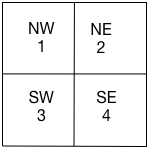
\includegraphics[scale=0.8]{Images/Childquad}
 \vspace{0.5in}
 \caption{NW - North west, NE - North east, SW - South west and SE - South east.}
 \label{fig:Childquad}
 \end{figure}

%%%%%%%%%%%%%%%%%%%%%%%%%%%%%%%%%%%%%%%%%%%%%%%%%%%%%%%%%%%%%%%%%%%%%%%%%%%%%%%
\section{Related Work}~\label{sec:relatedWork}
%%%%%%%%%%%%%%%%%%%%%%%%%%%%%%%%%%%%%%%%%%%%%%%%%%%%%%%%%%%%%%%%%%%%%%%%%%%%%%%

Traversal path for each polygon may differ, therefore linearizing the tree based on the traversal path for each polygon and iterating over the linear traversal order is computationally intensive.
Several application-specific approaches have been proposed to handle the problem.
 In algorithms like Barnes-Hut,  a point's traversal can be computed without executing the entire algorithm and a preprocessing pass can determine each point's linear traversal, avoiding repeatedly visiting interior nodes during vector operations. However, for PIP search, where a point's full traversal is only determined as the traversal progresses, the preprocessing step can be expensive.
 
Goldfarb et al. [2015]~\cite{goldfarb13sc} demonstrates a GPU implementation of tree traversal algorithms by installing ropes, extra pointers that connect a node in the tree not to its children,  instead to the next new node that a point would visit if its children are not visited. But the drawback of using ropes is that it requires an additional traversal prior to performing the actual traversals to create the ropes into the nodes of the tree structure. As a result, earlier attempts to use ropes to accelerate tree traversals have relied on application-specific transformations that leverage the semantics of the algorithm to efficiently place ropes.
The problem with using "Autoropes"~\cite{goldfarb13sc} is that since the rope pointers are computed during traversal and they are stored on the stack, it causes overhead due to stack manipulation and the efficiency is compromised.

Work by Zhang et al. [2013]~\cite{DBLP:journals/gis/ZhangY13} presents a speed up of 90x by constructing a quadtree using parallel primitives by transforming a multidimensional geospatial computing problem into chaining a set of generic parallel primitives that are designed for one dimensional arrays.

Another work by Bedorf et al. [2015]~\cite{Bedorf:2012:SOG:2133856.2134140} presents an octree construction where the tree is constructed on the GPU after mapping particles in 3D space to linear array. And a vectorized BFS traversal is done on the octree.

All of these implementations have relied on linearizing the tree for BFS traversal on the GPU or they have preprocessed the tree to either linearize or install extra pointers on the tree. 
CUDA GPU ray traversal through a hierarchical data structure such as a bounding volume hierarchy (BVH) is usually carried out using depth-first search by maintaining a stack.
This paper explores the parallelization of breadth-first search (BFS) to implement range search on GPUs. The kernel is optimized to minimize thread divergence and memory access. BFS is used instead of depth-first search (DFS) as it is easier to parallelize and implement efficiently on the GPU. BFS and DFS are fundamental building blocks for more sophisticated algorithms used in many computational fields that range from gaming, image processing to social network analysis. BFS is  used as a core computational kernel in a number of benchmark suites, including Rodinia, Parboil and the Graph500 supercomputer benchmark.

%%%%%%%%%%%%%%%%%%%%%%%%%%%%%%%%%%%%%%%%%%%%%%%%%%%%%%%%%%%%%%%%%%%%%%%%%%%%%%%
\section{Graphics Processing Unit Architecture}~\label{sec:gpu_overview}
%%%%%%%%%%%%%%%%%%%%%%%%%%%%%%%%%%%%%%%%%%%%%%%%%%%%%%%%%%%%%%%%%%%%%%%%%%%%%%%
%%%%%%%% GPU Hardware:
%DAC: GPU don't have cache, they are designed to exploit arithmetic intensity (high ratio of the number of arithmetic operations to the number of memory accesses).  Number of cores on a typical machine.  Use of shared memory has 1 cycle access and high-bandwidth for 16 threads per streaming multiprocessor).

The underlying architecture of the GPU is optimized for data-level
parallelism.  Taking a closer look at the
NVIDIA\textsuperscript{\textregistered} GPU reveals the chip is
organized into an array of highly threaded streaming multiprocessors 
(SMs). Each streaming multiprocessor consists of several streaming
processors (SPs). Streaming multiprocessors are grouped into thread
processing clusters (TPCs). The number of SPs per SM depends on the
generation of the chip.  

%TODO: Add GPU FLOPS vs CPU FLOPS chart?
NVIDIA\textsuperscript{\textregistered} has chips that increase the
number of streaming processors (SP) from 240 to 2048. Each SP has a
multiply-add unit plus an additional multiply unit.  The combined
power of that many SPs in this GPU exceeds one
teraflop~\cite{Kirk:2010:PMP:1841511}.  Each SM contains a special function
unit which can compute floating-point functions such as square root
and transcendental functions.  Each streaming processor is threaded and
can run thousands of threads per application.  Graphics cards are
commonly built to run 5,000-12,000 threads simultaneously on this GPU.
The GTX680 can support 192 threads per SMX and a total of 1536 threads
 simultaneously~\cite{nvidia:12:gtx680tech}. In contrast, the
Intel\textsuperscript{\textregistered} Core\texttrademark i7 series
can support two threads per core.

GPUs are optimized via the execution throughput of a massive number of threads.
The hardware takes advantages of this by switching to different threads while 
other threads wait for long-latency memory accesses.  This methodology enables
very minimal control logic for each execution thread~\cite{Kirk:2010:PMP:1841511}.
Each thread is very lightweight and requires very little creation overhead.

From a memory perspective, the GPU is architected quite differently
than a CPU.  Each GPU currently comes with up to four gigabytes of
Graphics Double Data Rate (GDDR) DRAM which is used as global
memory. The GPU architecture is designed to exploit arithmetic
intensity and data-level parallelism.

Figure~\ref{fig:KeplerArch} shows the architecture of the GTX680.
This generation of the CUDA enabled GPU devices consists of an array of 8 
next generation streaming multiprocessors (SMX), 4 GPCs and 4 memory controllers.
Each GPC has a dedicated raster engine and two SMX units.
Figure~\ref{fig:gpu_architecture} shows the architecture of a SMX. 
Each SMX unit contains 192 cores and four warp schedulers. 
Each warp scheduler is capable of dispatching two instructions per warp every clock~\cite{nvidia:12:gtx680tech}.

%  GPU picture
\begin{figure} [H]
    \centering
    \vspace{0.5in}
    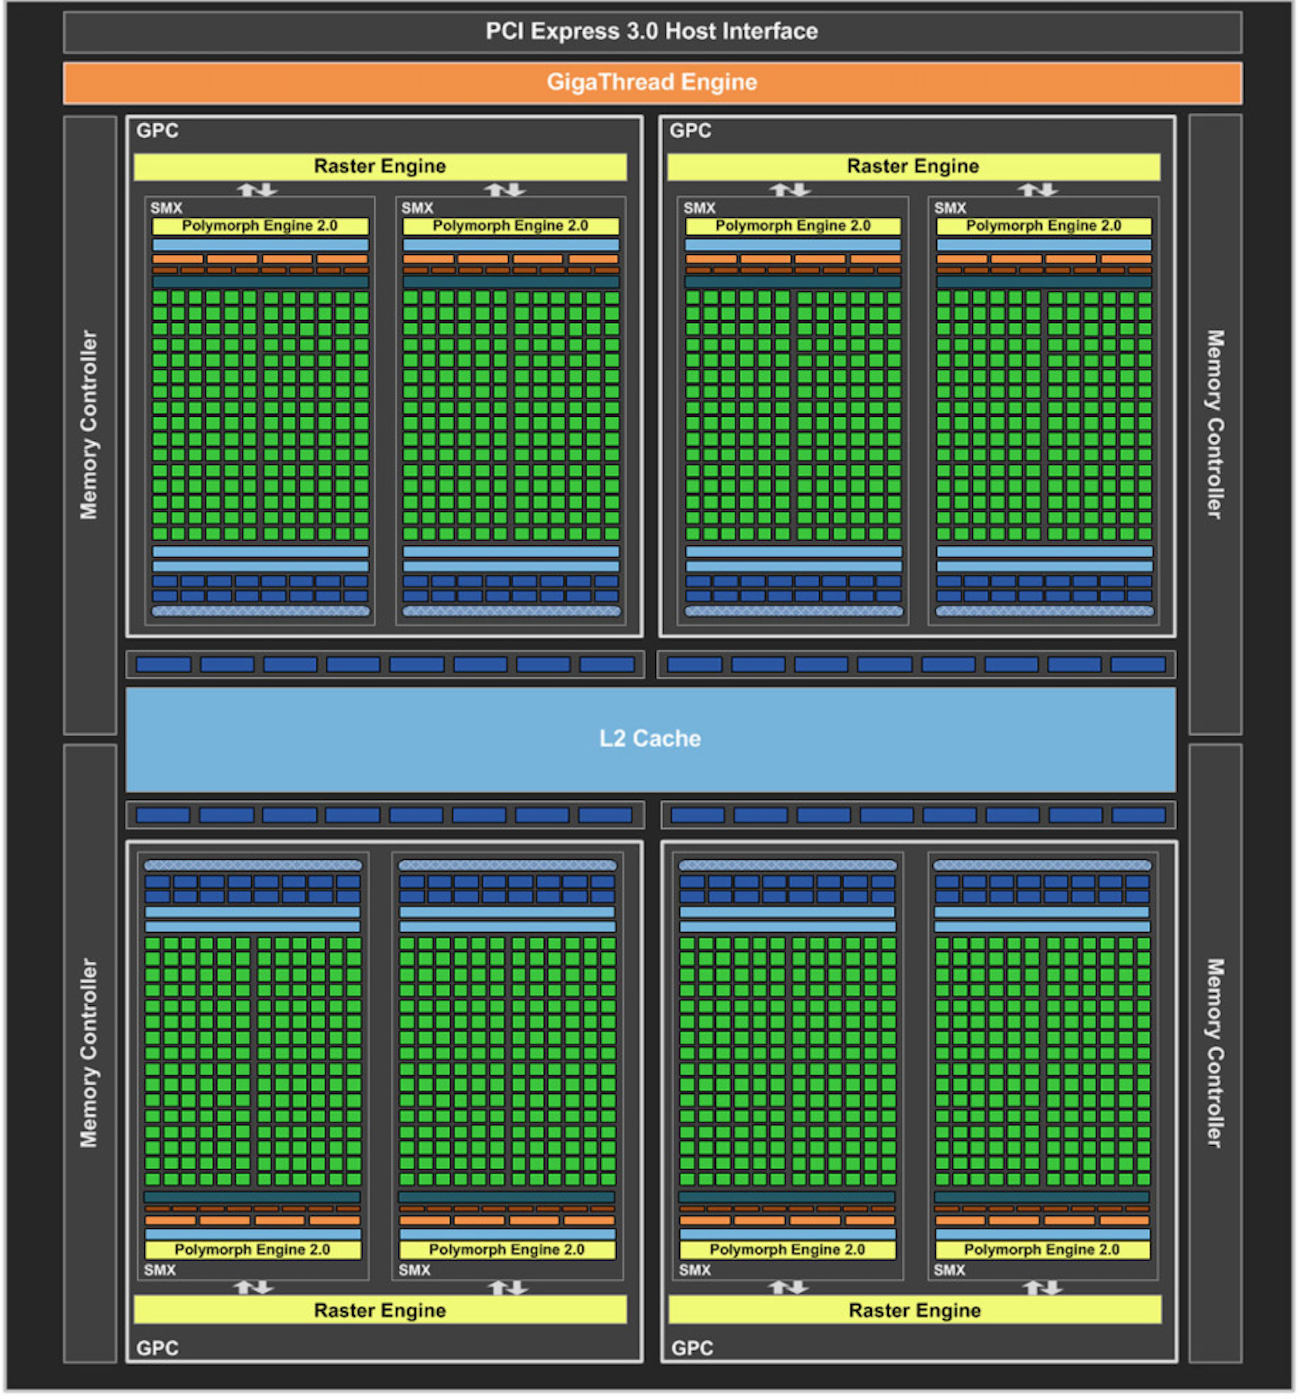
\includegraphics[scale=0.40]{Images/KeplerArch}
    \vspace{0.5in}
    \caption{Kepler Architecture.}
    \label{fig:KeplerArch}
\end{figure}

\begin{figure} [H]
    \centering
    \vspace{0.5in}
    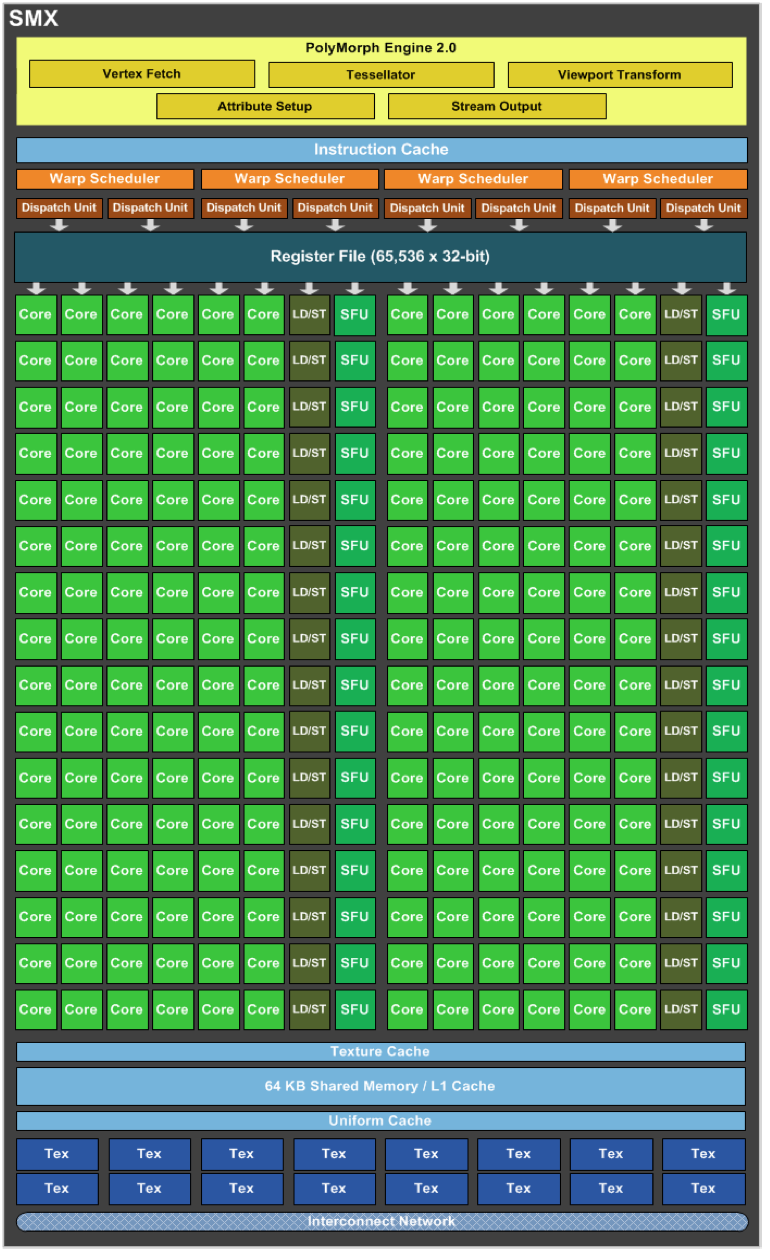
\includegraphics[scale=0.50]{Images/gpu_architecture}
    \vspace{0.5in}
    \caption{GTX680 SMX.}
    \label{fig:gpu_architecture}
\end{figure}

In Kepler, as shown in Figure~\ref{fig:memory}, each SMX has 64 KB of on-chip memory that can be configured as 48 KB of Shared memory with 16 KB of L1 cache, or as 16 KB of shared memory with 48 KB of L1 cache or a 32KB / 32KB split between shared memory and L1 cache.
In addition to the L1 cache, Kepler introduces a 48KB cache for data that is known to be read-only for the duration of the function and it also has a 1536KB of L2 cache memory.  The L2 cache services all loads, stores, and texture requests and provides high speed data sharing across the GPU~\cite{nvidia:12:gk110}.

\begin{figure} [H]
    \centering
    \vspace{0.5in}
    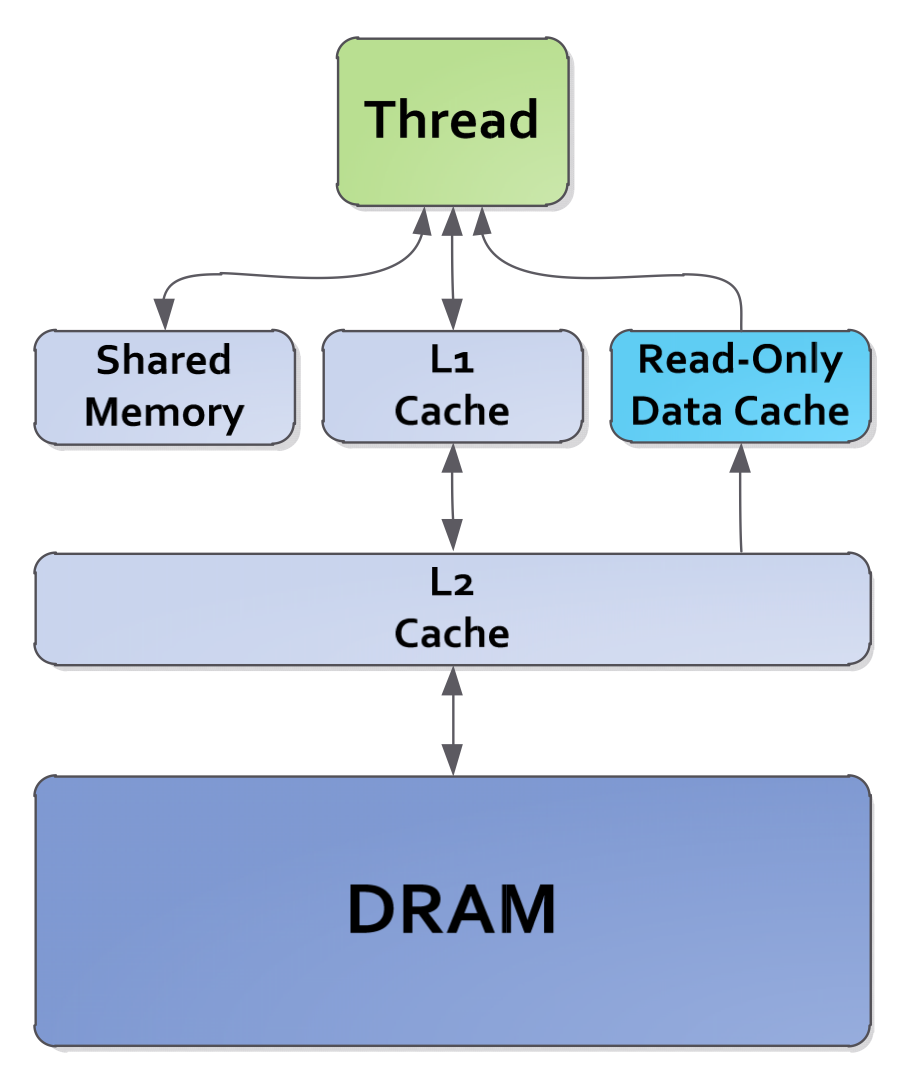
\includegraphics[scale=0.40]{Images/memory}
    \vspace{0.5in}
    \caption{Kepler Memory Hierarchy.}
    \label{fig:memory}
\end{figure}


%%%%%%%%%% GPU Interface (traditional vs CUDA)
%DAC:Must think in graphics terms to use
%    Restrictive programming models and instruction sets
%    Primitive tools Rapidly changing interfaces
Graphics processors have traditionally been designed for very specific
specialized tasks.  Most of their transistors perform calculations related
to 3D computer graphics rendering.  Typically GPUs perform memory-intensive
work such as texture mapping and rendering polygons.  The GPU also performs
geometric calculations such as rotation and translation of vertices into
different coordinate systems.  The on-chip programmable shaders can manipulate 
vertices and textures.  

NVIDIA\textsuperscript{\textregistered} has developed a parallel computing
architecture which is known as the Compute Unified Device Architecture (CUDA).  
This computing engine, which is the core of modern
NVIDIA\textsuperscript{\textregistered} GPUs, is accessible to software
developers through extensions of industry standard programming languages.  The
development of CUDA has enabled developers to access the virtual instruction
set and memory of the GPU. This has enabled the exploitation of the native
parallel computational elements of the NVIDIA\textsuperscript{\textregistered}
GPU. 

The Kepler architecture that has the Compute Capability 3.5 or higher supports dynamic parallelism, in which the GPU can launch new grids by itself. This feature allows algorithms that involve nested parallelism, recursive parallelism to be implemented on GPUs. This results in better GPU utilization than before. In Figure~\ref{fig:gpu_execution_hl_overview}, the Kepler host to GPU workflow 
shows the Grid Management Unit, which allows it to manage the actively 
dispatching grids, pause dispatch, and hold pending and suspended grids~\cite{nvidia:12:gk110}.

\begin{figure} [H]
    \centering
    \vspace{0.5in}
    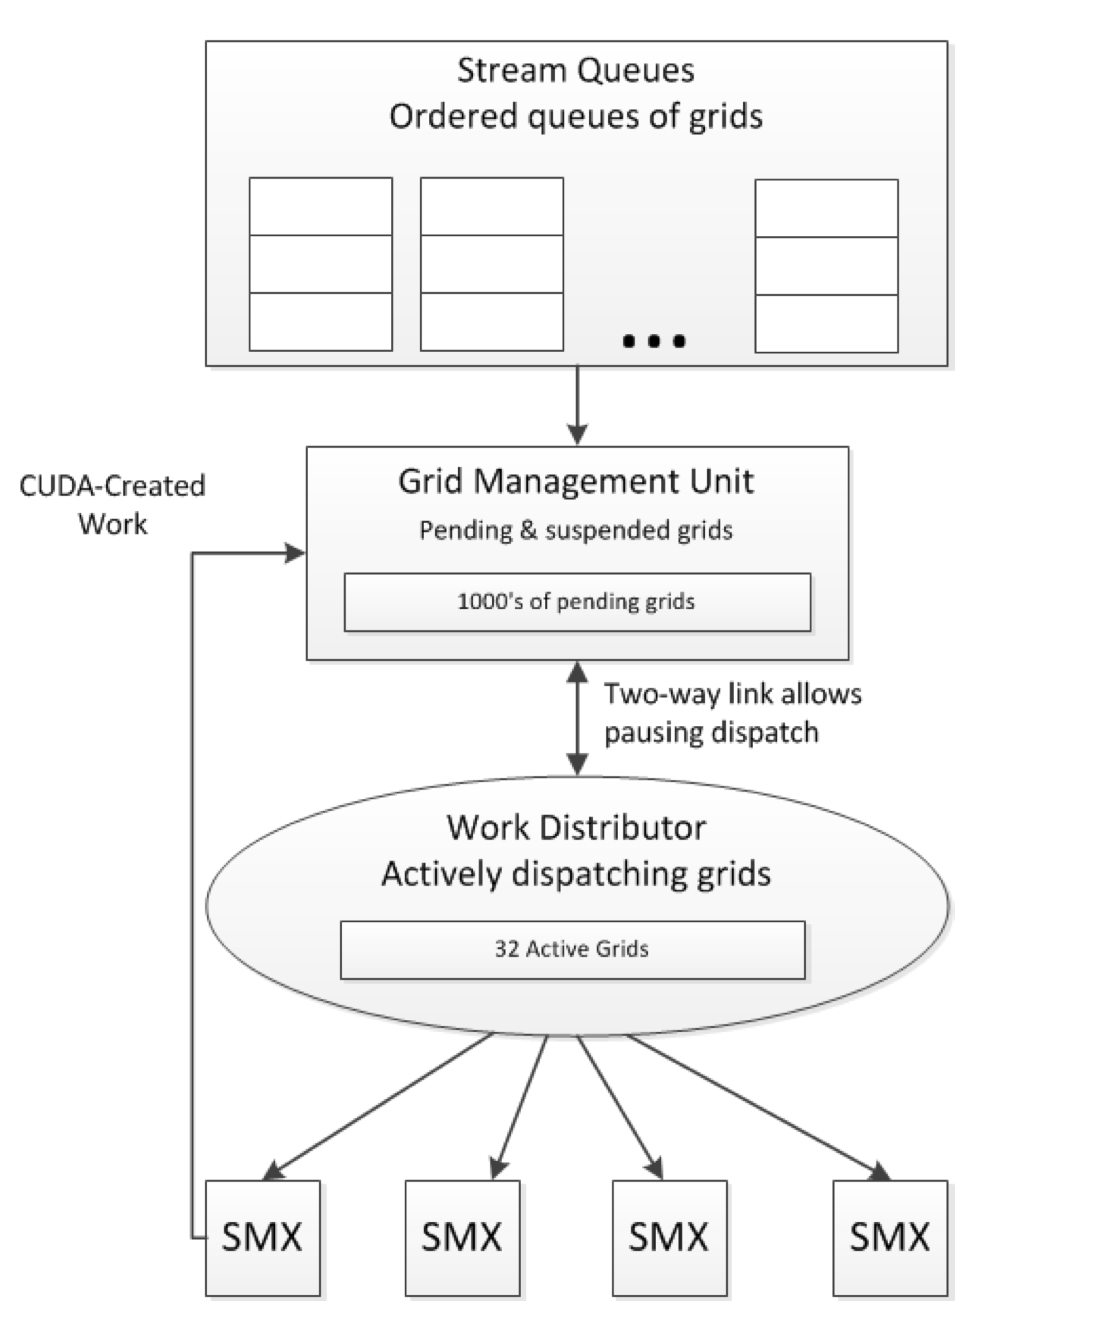
\includegraphics[scale=0.40]{Images/gpu_execution_hl_overview}
    \vspace{0.5in}
    \caption{Kepler Work Flow.}
    \label{fig:gpu_execution_hl_overview}
\end{figure}

%Scalablity and future compatibility

The CUDA model is optimized for maximum compatibility.
NVIDIA\textsuperscript{\textregistered} utilizes a soft instruction
set which enables the GPU designers to change the low level hardware
and instruction set without having to address backwards compatibility.
Similarly, NVIDIA\textsuperscript{\textregistered} has also built in
scalability to the CUDA model.  These GPUs are scalable in that the
CUDA code that is written is not tied to a specific release of the
NVIDIA\textsuperscript{\textregistered} GPU.  This can be contrasted
to traditional CPUs where the hard instruction set is published.  CPU
software developers often optimize their programs for how many cores
are available which can change as new CPUs are released.

A CUDA program
is comprised of multiple execution phases. Depending on the phase,
the execution involves the CPU, the GPU or both. Portions of the CUDA
code are executed on the GPU while other portions are executed on the
CPU.  The NVIDIA\textsuperscript{\textregistered} compiler known as
\textit{nvcc} translates the code for the GPU and CPU accordingly.
This model is very easy to work with because the device code is
written in ANSI C extended with keywords for labeling data-parallel
functions, called \textit{kernels}, and their associated data
structures~\cite{owens:08:gc}.

GPU implements a Single instruction multiple data (SIMD) model unlike the traditional CPU architectures where each thread may execute its own set of instructions. Multiple processing units are controlled by the same control signal from the control unit. Though each unit executes the same instruction, they have different data that corresponds to the CUDA threads.

 The GPU hardware maps the data blocks to the SMX through time and space multiplexing. Since each SMX has limited hardware resources such as shared memory, registers, number of threads that can be tracked and scheduled (scheduling lots), careful selection of block sizes allow the SMX to accommodate more blocks simultaneously thus increasing the throughput. 
 

%%%%%%%%%%%%%%%%%%%%%%%%%%%%%%%%%%%%%%%%%%%%%%%%%%%%%%%%%%%%%%%%%%%%%%%%%%%%%%%
\section{Motivation}~\label{sec:motivation}
%%%%%%%%%%%%%%%%%%%%%%%%%%%%%%%%%%%%%%%%%%%%%%%%%%%%%%%%%%%%%%%%%%%%%%%%%%%%%%%

In theory, for n items, the quadtree gives a performance of
${(n*log(n))}$. Compared to a brute force method's performance of
$n^{(2)}$~\cite{Eppstein:2000:FHC:351827.351829}, a quadtree is extremely fast. The performance gain by
using a quadtree is ${(log(n))/n}$.  As shown in
Figure~\ref{fig:comparing_bruteforce_cpu}, the empirical investigation
of quadtree search and brute force search shows that the quadtree has
a 9x better performance for medium number of queries and 8x
improvement for larger problems.  The main purpose of quadtree lies in
localizing the queries. The brute force search on a CPU checks
sequentially if every single point of the input data satisfies the
criteria whereas quadtrees help isolate the region of interest faster
by ignoring the quadrants of the tree that lie outside the region of
interest at every level, thus reducing the number of quadrants to be
processed at the next level. Therefore the quadtree gives better
performance for a dense more concentrated data than a dense equally
distributed data set.


\begin{figure}[H]
\centering
\vspace{0.5in}
    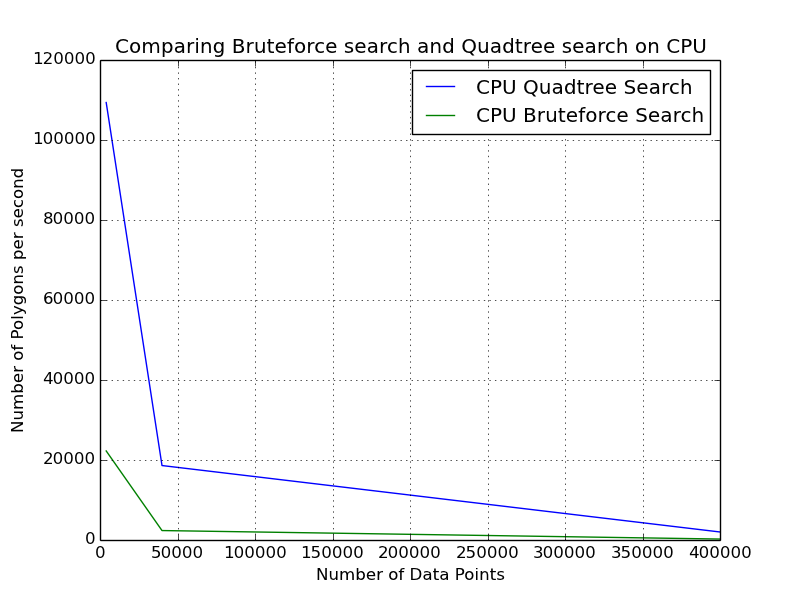
\includegraphics[scale=0.55]{Images/BruteVsQuadCPU_logscale_new_2}
    \vspace{0.5in}
    \caption{Comparing Bruteforce Search and Quadtree Search on CPU.}
    \label{fig:comparing_bruteforce_cpu}
  \end{figure}

As shown in Figure~\ref{fig:comparing_bruteforce_gpu}, the GPU provides a
better performance for brute force search compared to CPU for larger
datasets. But this performance is still lower than the CPU performance
using a quadtree. The same algorithm is used for both CPU and GPU
brute force search to check if a point is within the Polygon. But the
GPU is capable of launching 65535 blocks with a maximum of 1024
threads, thus massively parallelizing the search. The Geforce GTX680
Kepler architecture used, has a new parallel geometry pipeline
optimized for tessellation and displacement mapping. And also it has a
better performance / watt~\cite{nvidia:12:gtx680tech}.

\begin{figure}[H]
\centering
\vspace{0.5in}
    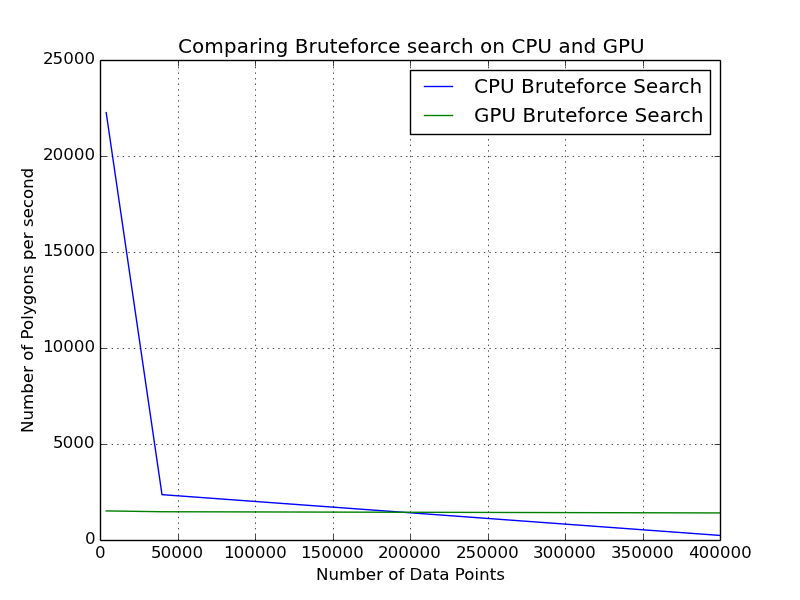
\includegraphics[scale=0.55]{Images/CPU_GPU_brute_new_2}
    \vspace{0.5in}
    \caption{Comparing Bruteforce Search on CPU with GPU.}
    \label{fig:comparing_bruteforce_gpu}
  \end{figure}

Figure~\ref{fig:cpu_quadtree_performance} shows the quadtree performance for different sized polygons. The small polygons occupy 10 to 20 percent of the quadtree area, the medium sized polygons occupy 30 to 60 percent of the quadtree area and the large polygons occupy 70 to 90 percent of the quadtree area.
The CPU implementation performs better on small polygons compared to larger polygons. The performance improvement in this case relates to how quickly the quadrants of the quadtree that contain the polygon can be isolated. The amount of computation done for a larger polygon that occupies all four quadrants is higher compared to a smaller polygon that lies inside only one quadrant.

\begin{figure}[H]
\centering
\vspace{0.5in}
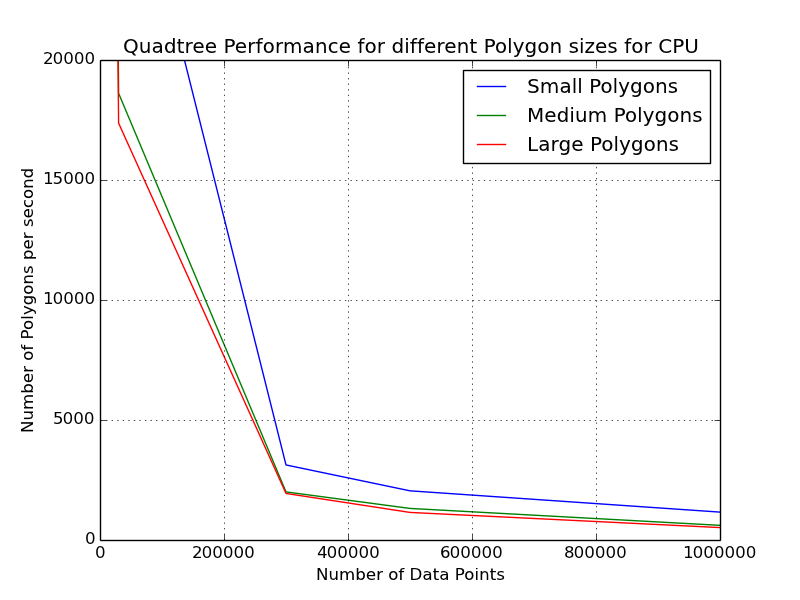
\includegraphics[scale=0.55]{Images/Different_Sized_Polygon_logScale_cpu04_10}
\vspace{0.5in}
\caption{CPU Performance of Different Sized Polygons using Quadtree.}
\label{fig:cpu_quadtree_performance}
\end{figure}


\chapter{Approach}\label{chap:approach}
%
% File - ch1.tex
%
%
% Description:
% This file should contain the first real chapter or section of your
% thesis.
%
%
%%%%%%%%%%%%%%%%%%%%%%%%%%%%%%%%%%%%%%%%%%%%%%%%%%%%%%%%%%%%%%%%%%%%%%%%%%%%%%%
\section{Exploitation of Quadtree on GPUs}
%%%%%%%%%%%%%%%%%%%%%%%%%%%%%%%%%%%%%%%%%%%%%%%%%%%%%%%%%%%%%%%%%%%%%%%%%%%%%%%

\subsection{CPU Implementation}

The traversal starts from the root node of the quadtree and performs DFS by recursion.
The traversal runs recursively till leaf node is reached. Depth First Search algorithm (DFS) traverses a graph in a depth wise motion and uses recursive function to get the next node to start a search when the bottom of the tree is reached. The traversal starts at the root node and moves down the tree till the bottom of the tree is reached along each branch before backtracking. While visiting each node, it checks for all three conditions to see if a node is completely overlapping,  partially overlapping or not overlapping.

Table~\ref{table:nonlin} illustrates the conditions to satisfy each scenario. N0, N1, N2 and N3 are the four corners of a node and the boundary of the polygon is marked by the four corners, P0, P1, P2, P3  of a rectangle. A checkmark indicates that the corner of the node is within the boundary of all four edges of a polygon. A x mark indicates that the corner of the node is outside the boundary of all four edges of a polygon.
If all the corners of a node is within the four edges of a polygon, then the node is completely overlapping the polygon. If all the corners of a node is outside the four edges of a polygon, then the node is not overlapping the polygon.
If at most three of the corners of a node is outside the four edges of a polygon, then the node is partially overlapping the polygon. All the conditions apart from the ones shown in Table 1 are partially overlapping.

\begin{table}[H]
\centering\begin{tabular}{c c c c c c}
\hline\hline
Case & N0 & N1 & N2 & N3 & Condition \\ [0.5ex] % inserts table 
%heading
\hline
P0 P1 P2 P3 & \checkmark & \checkmark & \checkmark & \checkmark & Completely overlapping \\
P0 P1 P2 P3 & \xmark & \xmark & \xmark & \xmark & Not overlapping \\
\hline
\end{tabular}
\caption{Criteria for Quadtree Node Classification.}
\label{table:nonlin}
\end{table}

Before classifying the node as not overlapping, the polygon is also checked to see if it lies inside the node. If the node is classified as completely overlapping node, then the boundary details of this node is stored and tree is not traversed further from this node. The boundary of the node represents the range of points the node contains and all these points within the node are considered as points within the polygon.
If the node is classified as not overlapping node, then the tree is not traversed further from this node. 
If the node is classified as partially overlapping  node then the tree is traversed further till the leaf node is reached. The points are then extracted from the leaf nodes of the quadtree.

In the case of partially overlapping node, every point needs to be checked to see if it lies within the boundary of the polygon. This check is optimized by classifying the kind of intersection between the node  and the Polygon in such a way that for certain scenarios only either x or y coordinate of the points need to be verified. 

If the intersection of the node is along the horizontal edge of the polygon as in Figure~\ref{fig:overlap2}, then only the y coordinate of the data points inside the node needs to be checked as all the x-coordinate of all points is within the polygon boundary limits. If the intersection between the node and the polygon is along the vertical edge of the polygon as in Figure~\ref{fig:overlap3}, then only the x coordinate of the points needs to be checked as all the y-coordinate of all points is within the polygon boundary limits. For all the other overlap conditions, x-y coordinate of every point is checked with the boundary limits of the polygon.

\begin{figure}[H]
\centering
\vspace{0.5in}
\includegraphics[scale=0.8]{Images/OverlapScenario4}
\vspace{0.5in}
\caption{Overlap of Node on the Horizontal Edge of Polygon.}
\label{fig:overlap2}
\end{figure}

\begin{figure}[H]
\centering
\vspace{0.5in}
\includegraphics[scale=0.8]{Images/OverlapScenario5}
\vspace{0.5in}
\caption{Overlap of Node on the Vertical Edge of Polygon.}
\label{fig:overlap3}
\end{figure}

In the case of GPU implementation, x-y coordinates of all points of the partial node are checked against the polygon edges without classifying them based on the type of node intersection as it will lead to more conditional statements which would increase thread divergence and reduce the performance.

\subsection{GPU Implementation}

Efficient implementation of quadtree traversal in GPU using CUDA is challenging due to the following reasons. 1. The quadtree is an irregular data structure whose memory accesses and work distribution are both irregular and data-dependent. And traversing irregular data structures results in thread divergence.
2. Traversal of a quadtree built using pointers results in lot of pointer-chasing memory operations. Pointer-chasing leads to many un-coalesced memory accesses which affects performance~\cite{barnes:hut}.
3. As done typically the quadtree is built using recursive depth first style in the CPU. Recursive DFS in GPU would be advantageous as it will reduce un-coalesced memory accesses considering the memory for all the structures is preallocated. Recursion can be implemented only on the latest GPUs with CUDA 6.5 version that supports dynamic parallelism, but recursion could lead to low performance due to function call overhead. Recursion on a GPU, requires explicit stack space per thread and deep recursion will cause overflow of the available stack space and in this case CUDA may reduce the maximum physical threads per launch.
4. Transferring a pointer based quadtree to a GPU proves to be a challenge. Though this task can be implemented with "cudamallocamanaged" function, debugging becomes harder.

To take advantage of the parallel nature of the GPUs, BFS is used instead of DFS. 
The quadtree is queried to find the points inside a polygon by first finding the quadtree nodes that overlap the polygon. Once the nodes that overlap the polygon are determined, the points inside the polygon can be found from these nodes. Given a set of nodes, arranged hierarchically, the system needs to find the minimum set which solves the query correctly. This can be done by assigning one thread to a polygon but there is not enough stack space. Since our GPU implementation method requires an explicit array in the shared memory for each polygon, assigning one thread to a polygon will also pose a limit on the number of polygons processed simultaneously by a block due to the limitation in the shared memory size.
The stack space per thread needs to be reduced and optimization for thread divergence and memory access should be done. To minimize thread divergence and reduce stack space per thread and also achieve maximum parallelization, a polygon is assigned to a warp instead of a thread or a block of threads. To optimize for memory access, memory preallocation for the input points, query polygons, point buffer (list that holds points within a leaf node of quadtree) is done on the CPU.

CUDA applications exploit massive data parallelism and it is capable of processing massive amount of data within a short period of time. But data accesses to GDDR DRAM global memory limits this performance due to limitations in global memory bandwidth. Therefore algorithms and techniques need to be employed in order to reduce the demand on the DRAM bandwidth  and make efficient use of the data accessed from the global memory~\cite{Kirk:2010:PMP:1841511}.


The quadtree is built on the CPU from heap objects and each heap object has several fields. For example, each quadtree node object contains 4 child pointers and  data fields which stores the attributes of the node. Other heap objects include data points and point buffers. 
Though the CPU implementation benefits from the dynamic memory allocation, the use of the C library malloc is not preferred for the CPU-GPU implementation because this dynamic memory-management function provides allocation and de-allocation of arbitrary segments of memory. In order to improve performance on the GPU, the access to memory segments need to be coalesced. The memory preallocation places the consecutive points and point buffers sequentially in memory and therefore results in memory coalesced access as the points close to one other are more likely to be within the same polygon boundary. But preallocating memory for the  quadtree nodes is not expected to improve performance as the nodes are stored in a depth first fashion in the CPU but a BFS traversal is done on the GPU.

The DRAM cores are slower as the market demands a high capacity rather than a lower latency DRAM.  These cores operate at much lower speed compared to the interface speed. GDDR4 operates at 1/8th of the interface speed and this difference will increase with every generation of GDDR as the storage capacity increases~\cite{Kirk:2010:PMP:1841511}.
Since DRAM cores are slower than the interface, the system needs to increase the buffer width to feed into faster interface. The modern DRAM banks are designed to be accessed in burst mode. If the accesses are not to sequential locations, the transferred burst bytes are discarded.
In order to take full advantage of the DRAM system in CUDA environment, the system needs to make sure that the processor makes use of all the data bursted out of the DRAM chip.
Thus from a memory throughput standpoint to get peak memory performance, computation must be structured around sequential memory accesses~\cite{Kirk:2010:PMP:1841511}. Random memory access leads to a huge performance penalty due to random memory reads.


\subsubsection{Drawbacks on implementing DFS on GPU}

One option to traverse down the tree for every polygon is to use DFS by assigning a warp or a thread to each polygon. But the DFS implementation in the GPU would cause a overhead due to the data movement as the thread moves up and down the tree. In this case the interior nodes of the tree are repeatedly visited as a thread has to return to higher level of the tree to traverse down to other children~\cite{goldfarb13sc}. This results in additional work for each thread.

\subsubsection{BFS Implementation on GPU}


Stack based breadth first tree-traversal allows parallelization. To take advantage of the parallel nature of the GPU, the threads are launched at level 3 of the quadtree instead of the root node. Starting at the root node will result in only one thread being active for level 1 traversal of quadtree. Starting at a deeper level prevents this and results in more parallelism.
Initially the index of the node from level 3 of the quadtree is stored in an array in the shared memory.
This index is used to fetch the quadtree node from the global memory.

Here the tree is traversed down to find the boundaries of a polygon and thus extracting the quadtree nodes within that boundary or partially overlapping the boundary. For completely overlapping nodes, the boundary of the node gives the range of points within the polygon. This method is more efficient than traversing down the quadtree to find the individual points within the polygon in terms of computation and also memory. And for partially overlapping nodes, each point needs to be checked against the boundary of the polygon. With this information, the range of points within the polygon region can be found and this range is stored instead of individual points to save memory on the GPU. If there are a very large number of input points and query polygons, then storing individual points for each polygon will result in overflow of the memory. 

The Polygons are associated with a CUDA warp, where the number of threads in a warp depends on CUDA configuration. By launching thousands of GPU blocks in parallel, 'N' number of polygons can be queried, where N = (size of each block / 32)*(total number of blocks).  Each warp executes the same algorithm but on a different polygon. Assigning a warp to a polygon will result in less thread divergence. Each thread in a warp reads x, y co-ordinate of all four corners of a polygon which is required for the tree traversal.

The GPU kernel replaces the recursive call with stack push operations that save indices of each child of a node traversed, that satisfies the query. Traversal is facilitated by a loop that simultaneously assigns the indices of the nodes in the stack to threads in warp until the stack is empty, indicating there are no more nodes to visit at that level for a polygon. To save stack space, node indices are stored in the stack instead of the node. At the beginning of each iteration of the loop the nodes are popped from the stack. After popping the node from the stack, the function which checks for the overlapping conditions is executed on that node, possibly pushing more nodes onto the stack or returning when it reaches a node that fails the criteria, an empty node or a leaf node.

If the number of nodes in the stack exceeds the number of threads assigned to a polygon, then loop over with increments of the number of threads in a warp is done. Within each loop, each node is assigned to one thread.
Each thread reads the quadtree node's properties and tests whether or not to traverse the tree further down from this node. If the criteria to traverse the tree down from this node is satisfied, then the indices of the node's all four children is added to the stack, provided the child is not an empty node. One stack space is assigned to each polygon. Traversal at each level of quadtree is synchronized, so that the same stack can be re-used for a polygon. The tree-traverse loop is repeated until all the levels of the quadtree is visited.
The number of GPU threads used per level is equal to the number of nodes that was pushed on to the stack from the previous iteration.

The warp starts the traversal at level 3 of the quadtree. The indices of children of the nodes that satisfy the query are placed in an array. The condition checks whether a node is overlapping the polygon. Once the indices of children of the nodes that satisfy the query are placed in an array and the other nodes, which do not satisfy the condition are ignored, the next level is evaluated.
Once the leaf node is reached, the nodes are classified as completely and partially overlapping nodes. And from these nodes all the points that are inside the Polygon are taken. The boundaries of the completely overlapping nodes which give the range of points within the nodes are stored.

In the case of partially overlapping nodes, each point within the node is checked against the boundary of the polygon and the range of points that lie within the polygon is stored. At the last level of the tree, the warp still holds the polygon and the threads within a warp is assigned to a leaf node that is either partially or completely overlapping the polygon. Each of these threads compute the points within each node that are inside the polygon.

This approach will minimize the use of shared memory space, as only the indices of nodes are stored starting from level 3 in shared memory instead of the node itself that satisfy the required criteria. The indices of the nodes are used to fetch the corresponding node from the global memory.
The order in which the nodes are stored in the stack does not matter, as every level in the quadtree is processed independent of the previous and every node is processed independent of other nodes in the stack.

The indices of the nodes are saved in the stack array in the shared memory and the the stack is cleared after computing every level. Shared memory blocks are used in order to gain significant speedups of approximately 150 to 200 times~\cite{Kelly:gpu}. If a node index returns -1, then the node is empty and it is not fetched from the global memory.
The number of nodes that needs to be visited  at the next level is also stored in a shared memory variable for every polygon and it is incremented atomically. The iterative loop launches threads based on the count on this variable. The loop executes till the last level of quadtree is reached.

To implement this algorithm, the maximum number of levels in a quadtree should be 4 because of the limitations in the size and the number of stacks in the  shared memory. As the number of levels in a quadtree increases, the maximum stack space required per polygon would also increase and this will limit the number of polygons processed.

The size of shared memory per block on the GTX680 is 49152 bytes~\cite{nvidia:12:gtx680tech}. As there are 32 warps in a block by default, each block is assigned  32 polygons. Each polygon requires an array in the shared memory in order to store the node indices from each level that needs to be further traversed. The maximum array size required for a 4 level quadtree is 64 as the maximum number of nodes at the leaf is 64. This allocation occupies a shared memory space of 32 * 64 *4 = 8192 bytes, which is well within the limit. The array size for each polygon needs to be increased to 256 for a 5 level quadtree. This allocation results in a shared memory usage of 256 * 32 * 4  = 66560 bytes, which exceeds the available shared memory size. Therefore unless a larger size of shared memory becomes available in the future, the quadtree cannot not be subdivided beyond level 4 in this case.

In Figure~\ref{fig:bfs_gpu}, the check mark indicates that the node  satisfies the query and the tree will be further traversed from this node. The cross mark indicates either that the node does not satisfy the query or the node is empty and the threads terminate at this point without proceeding further.

\begin{figure}[H]
\vspace{0.5in}
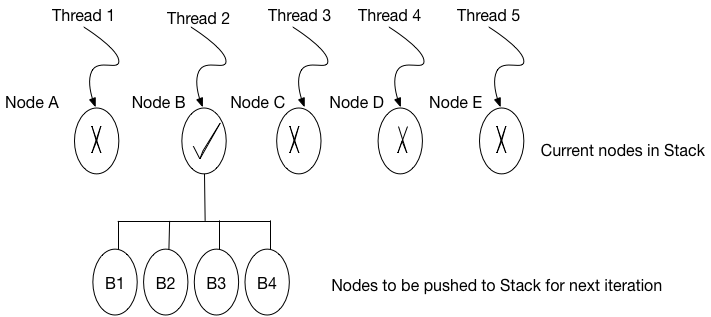
\includegraphics[scale=0.5]{Images/BFSgpu}
\vspace{0.5in}
\caption{BFS GPU Implementation.}
\label{fig:bfs_gpu}
\end{figure}

The traversal starts at level 3 of the quadtree. The children of the nodes that satisfy the overlap conditions are pushed in to the array. The array is initialized after every iteration. 
The cross mark indicates that the node is either not satisfying the overlap conditions or it is empty. The nodes are stored in the array in any order. The process repeats till bottom of the tree is reached. 
The number of stack array in the shared memory per block depends on the number of warps in a block. At the most, the iterative loop processes 32 nodes at a time by default (equal to the number of threads in a warp). The conditional statements are changed to avoid function return statements to prevent the traversal loop from prematurely exiting and preventing the remainder of the loop body from executing.

A polygon is checked against the node of the quadtree for 3 scenarios such as, completely overlapping,  partially overlapping and not overlapping.
All nodes are checked for "not overlapping" conditions till leaf node is reached. If a node satisfies the condition then the tree is not traversed from this node and if the node does not satisfy the condition, then its children are placed in the stack and the traversal continues.

The number of checks for a partially overlapping node is more and use of "if" statements decreases the performance due to control divergence. If threads within a warp take different paths, then 2 passes on the different path of the code is required to execute all threads. Since different execution paths are serialized, it leads to performance penalty.

Therefore in order to reduce conditional statements (if statements), the condition for completely overlapping node is first computed on the leaf nodes and the nodes that satisfies the condition is classified as completely overlapping nodes and nodes that does not satisfy the condition is classified as partially overlapping nodes. The Figure~\ref{fig:FlowChart}, shows the high level overview of the algorithm to find the points in polygon using quadtree on a GPU. 

\begin{figure}[H]
\centering
\vspace{0.5in}
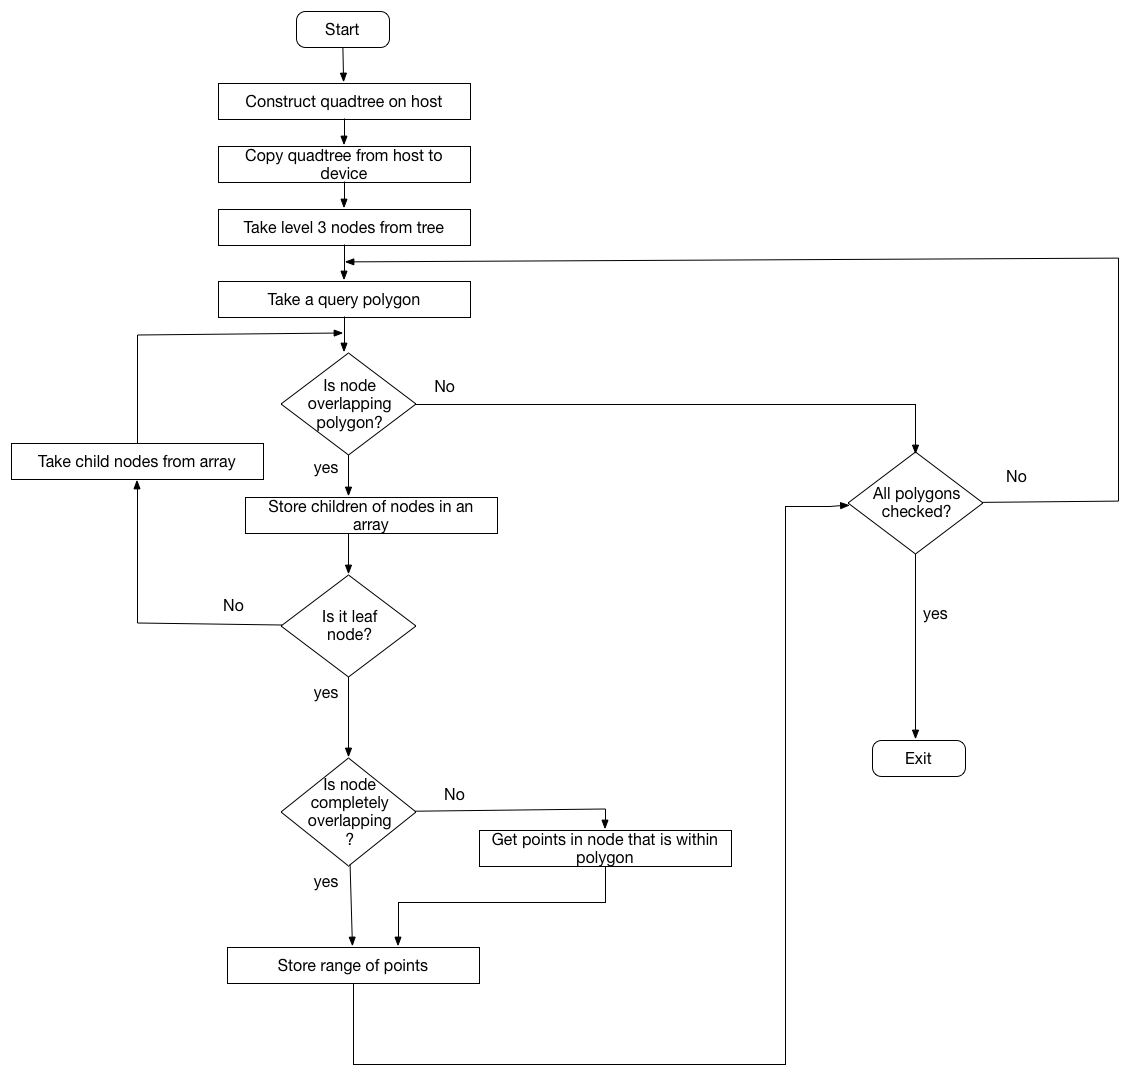
\includegraphics[scale=0.35]{Images/FlowChart}
\vspace{0.5in}
\caption{Process Flow.}
\label{fig:FlowChart}
\end{figure}

\subsection{BFS Implementation on GPU - Different Scenarios of Query Polygon}

The Figure~\ref{fig:level1quadtree}, Figure~\ref{fig:level2quadtree}, Figure~\ref{fig:level3quadtree} and Figure~\ref{fig:level4quadtree} show the data points (left)  and its corresponding tree representation (right). These data points will be analyzed for different polygon overlap scenarios in the next sections.
The numbers inside the circle represent the index of the node at that level.
Figure~\ref{fig:level1quadtree} shows the root node that contains all input data points. The root node is subdivided into 4 equal regions to form 4 nodes at level 2.
Figure~\ref{fig:level2quadtree} shows the four children of the root node. Root node has all four children as the data points are present in all four directions (NW, NE, SW, SE) of the root node. The nodes at level 2 are again subdivided equally to form the child nodes.
Figure~\ref{fig:level3quadtree}, shows the nodes at level 3 of the quadtree. Child node 3 of parent node 1 from level 2, child node 1 and child node 4 of parent node 3 from level 2 and child node 3 of parent node 4 from level 2 are empty as the parent nodes did not have any points in those directions.
Figure~\ref{fig:level4quadtree} shows the child nodes at level 4. Many of the nodes at this level are empty as they do not contain any points.


\begin{figure}[H]
  \centering
  \vspace{0.5in}
  \begin{minipage}[b]{0.35\textwidth}
    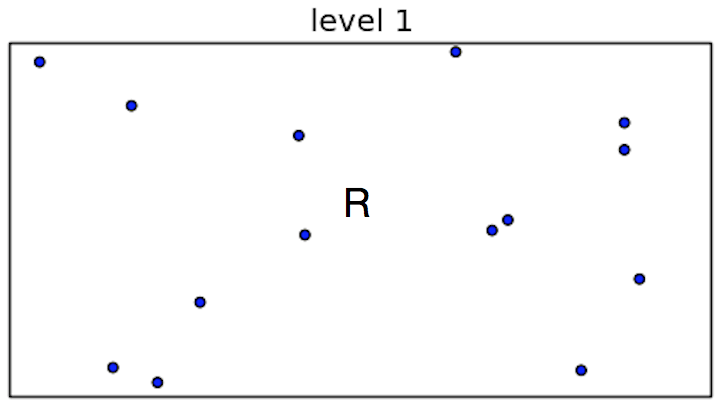
\includegraphics[width=\textwidth]{Images/Quadtree_basic_scenario6}
  \end{minipage}
  \hfill
  \begin{minipage}[b]{0.4\textwidth}
    
\includegraphics[width=\textwidth]{Images/R1}
  \end{minipage}
  \vspace{0.5in}
  \caption{Level 1 Quadtree.}
  \label{fig:level1quadtree}
\end{figure}

\begin{figure}[H]
  \centering
  \vspace{0.5in}
  \begin{minipage}[b]{0.35\textwidth}
    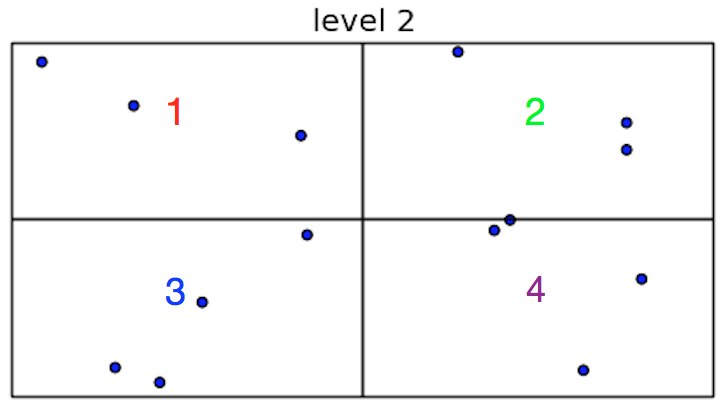
\includegraphics[width=\textwidth]{Images/Quadtree_basic_scenario7}
  \end{minipage}
  \hfill
  \begin{minipage}[b]{0.6\textwidth}
    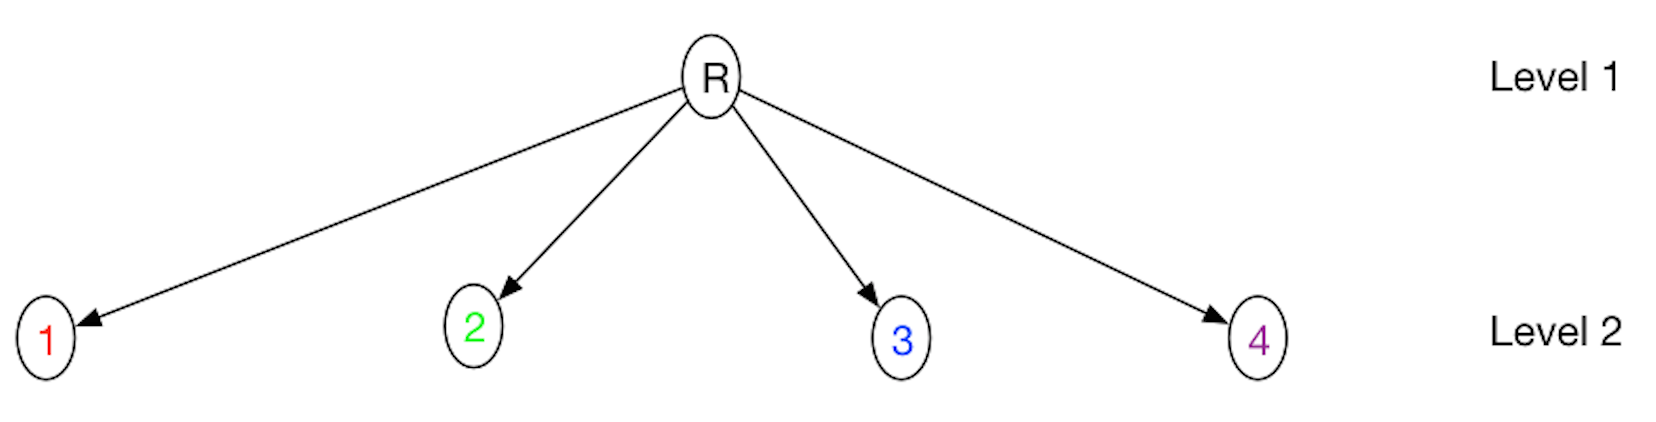
\includegraphics[width=\textwidth]{Images/L2_Tree}
  \end{minipage}
  \vspace{0.5in}
  \caption{Level 2 Quadtree.}
  \label{fig:level2quadtree}
\end{figure}

\begin{figure}[H]
  \centering
  \vspace{0.5in}
  \begin{minipage}[b]{0.35\textwidth}
    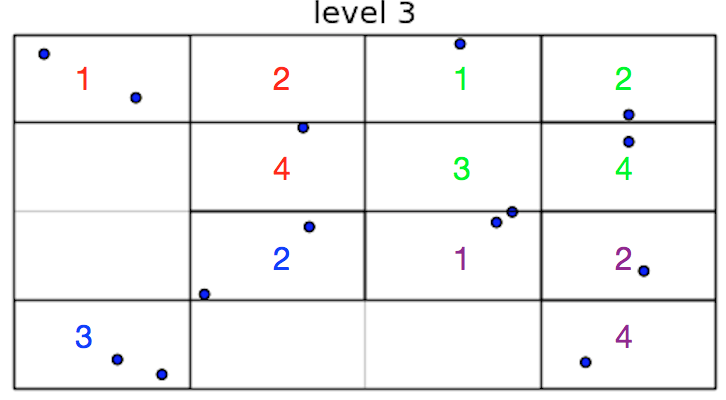
\includegraphics[width=\textwidth]{Images/Quadtree_basic_scenario8}
  \end{minipage}
  \hfill
  \begin{minipage}[b]{0.6\textwidth}
    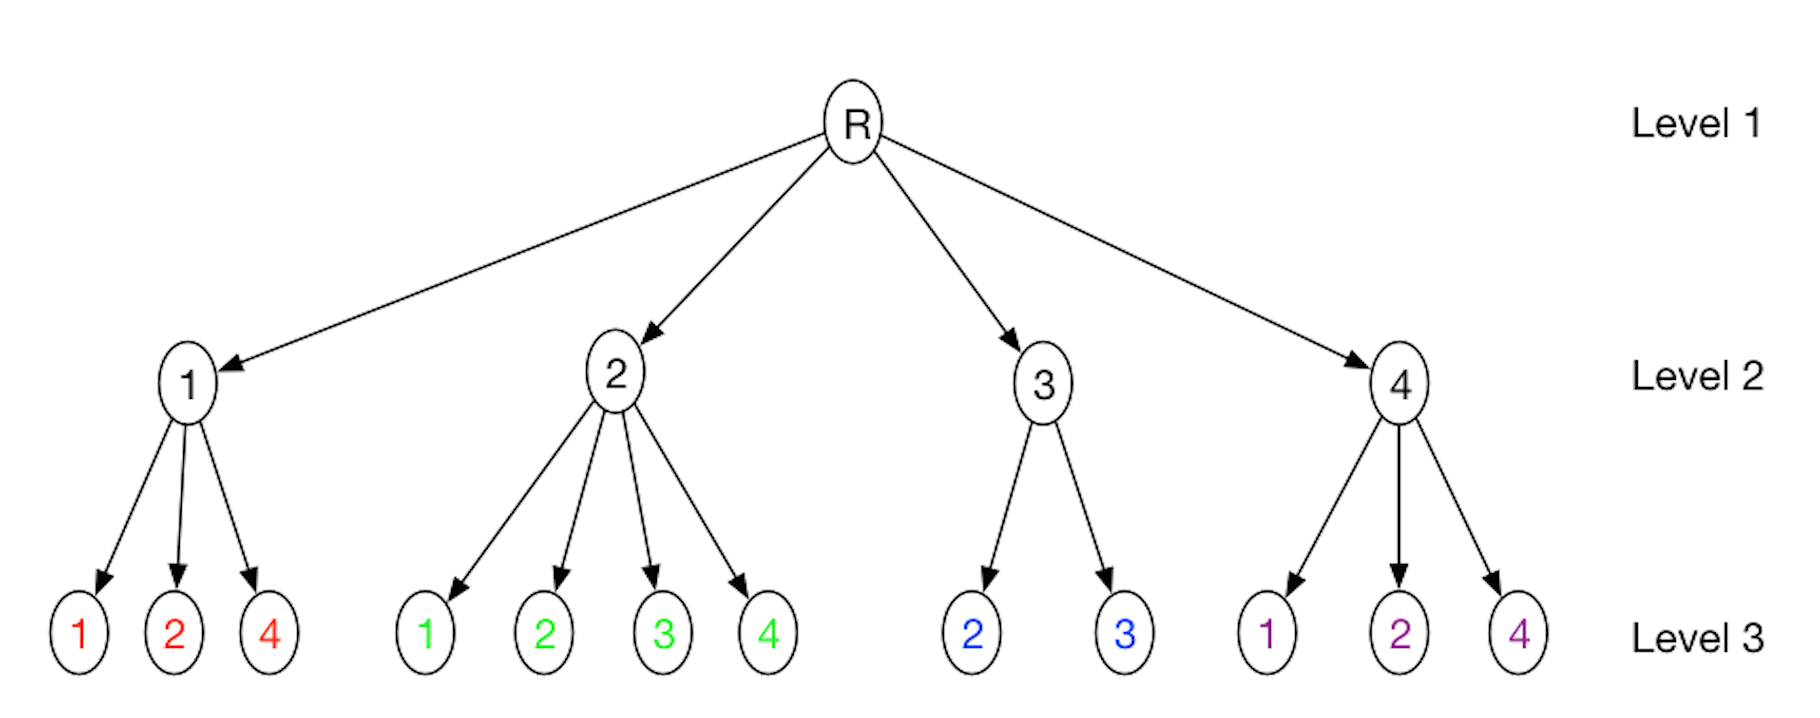
\includegraphics[width=\textwidth]{Images/L3_Tree}
  \end{minipage}
  \vspace{0.5in}
  \caption{Level 3 Quadtree.}
  \label{fig:level3quadtree}
\end{figure}

\begin{figure}[H]
  \centering
  \vspace{0.5in}
  \begin{minipage}[b]{0.35\textwidth}
    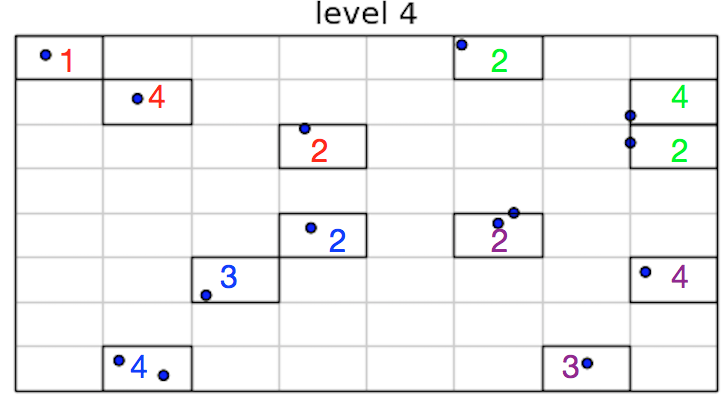
\includegraphics[width=\textwidth]{Images/Quadtree_basic_scenario9}
  \end{minipage}
  \hfill
  \begin{minipage}[b]{0.6\textwidth}
    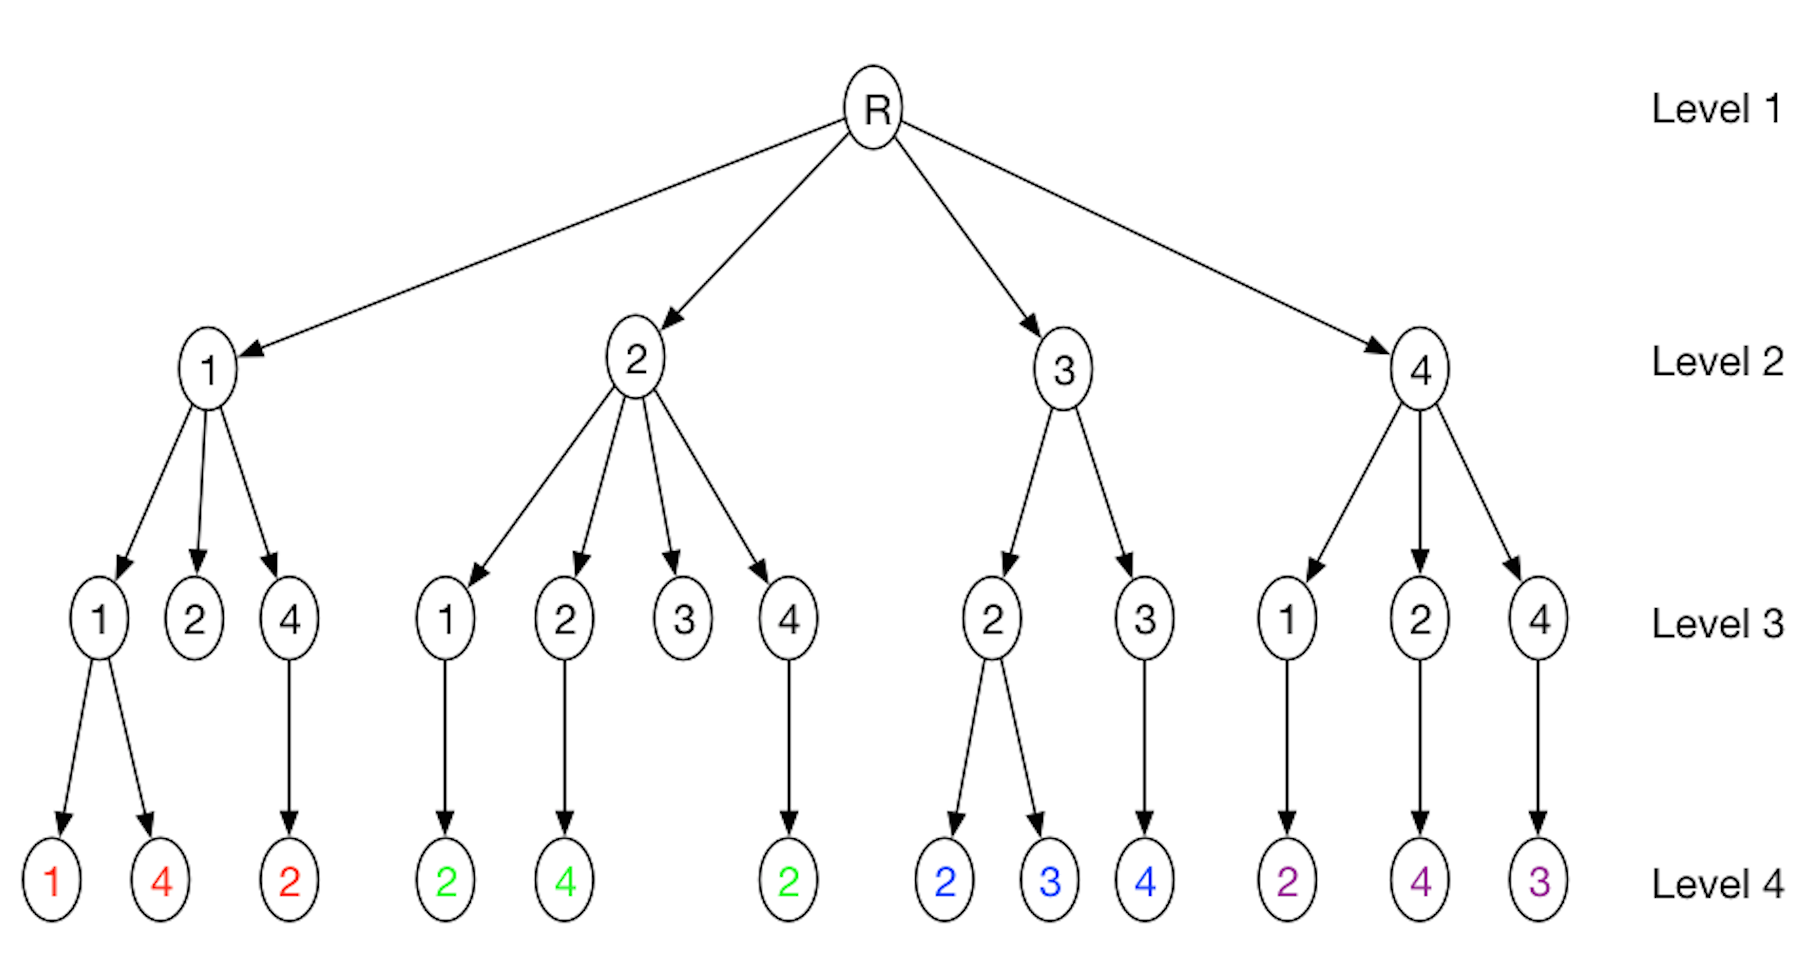
\includegraphics[width=\textwidth]{Images/L4_Tree}
  \end{minipage}
  \vspace{0.5in}
   \caption{Level 4 Quadtree.}
  \label{fig:level4quadtree}
\end{figure}

\clearpage
\subsubsection{Query Polygon inside a Leaf Node}

Figure~\ref{fig:Level1} shows the first scenario that demonstrates the best case scenario where the polygon lies within one quadrant at level 4 of the quadtree and the algorithm provides best performance.

\begin{figure}[H]
  \centering
  \vspace{0.5in}
  \begin{minipage}[b]{0.35\textwidth}
    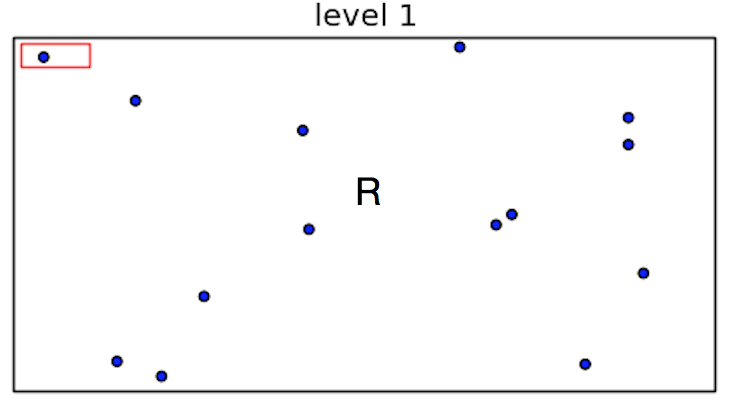
\includegraphics[width=\textwidth]{Images/1_1Quad1_1}
  \end{minipage}
  \hfill
  \begin{minipage}[b]{0.5\textwidth}
    
\includegraphics[width=\textwidth]{Images/1_1Quad_1_tree}
  \end{minipage}
  \vspace{0.5in}
   \caption{Sample Datapoints (left) and the Quadtree (right) at Level 1.}
   \label{fig:Level1}
\end{figure}


Figure~\ref{fig:Level2} shows that at level 2, the algorithm isolates one quadrant (first child of the root node) and ignores all other quadrants, thus bringing down the number of quadrants to be processed to 1 from 4 (4 is the total number of nodes at this level).

\begin{figure}[H]
  \centering
  \vspace{0.5in}
  \begin{minipage}[b]{0.35\textwidth}
    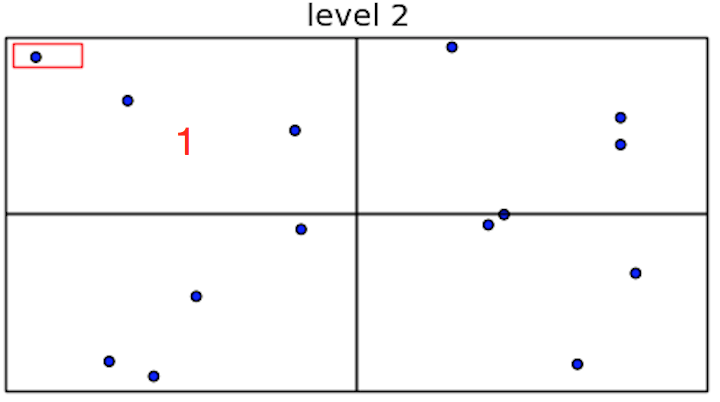
\includegraphics[width=\textwidth]{Images/1_1Quad1_2}
  \end{minipage}
  \hfill
  \begin{minipage}[b]{0.5\textwidth}
    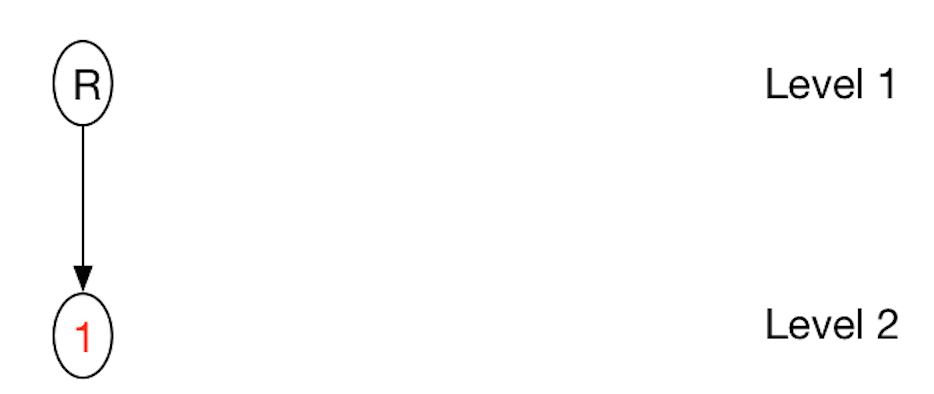
\includegraphics[width=\textwidth]{Images/1Quad_2_tree}
  \end{minipage}
  \vspace{0.5in}
  \caption{Sample Datapoints (left) and the Quadtree (right) at Level 2.}
   \label{fig:Level2}
\end{figure}

Figure~\ref{fig:Level3} shows that at level 3, the algorithm again isolates one quadrant which is the first child of the quadrant from level 1. This step reduces the number of quadrants to be processed to 1 from 3 (3 is the total number of children of the node output from level 1).

\begin{figure}[H]
  \centering
  \vspace{0.5in}
  \begin{minipage}[b]{0.35\textwidth}
    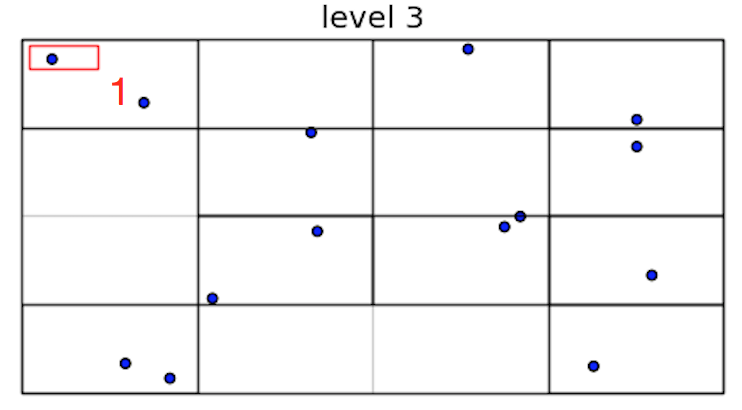
\includegraphics[width=\textwidth]{Images/1_1Quad1_3}
  \end{minipage}
  \hfill
  \begin{minipage}[b]{0.5\textwidth}
    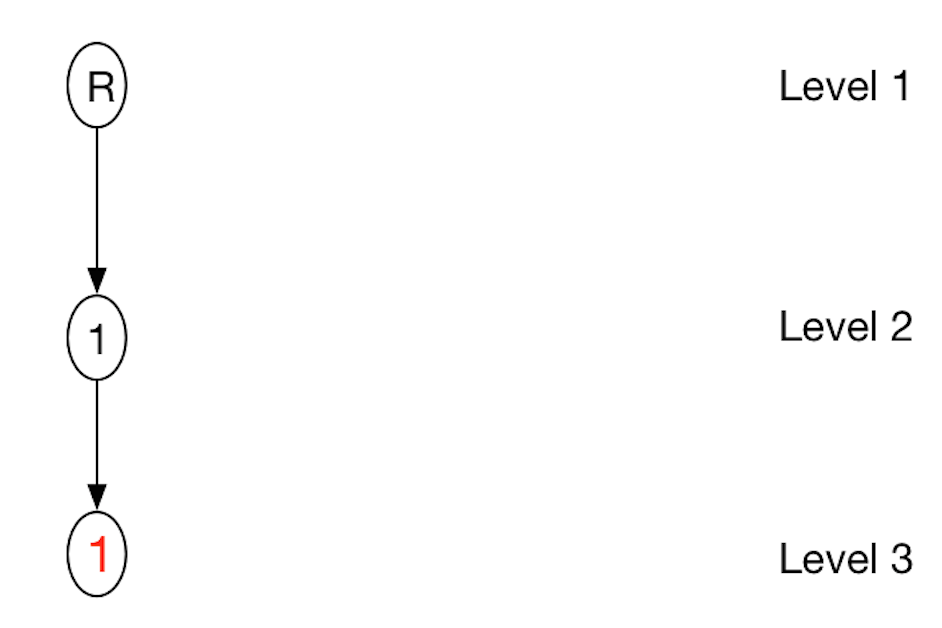
\includegraphics[width=\textwidth]{Images/1Quad_3_tree}
  \end{minipage}
  \vspace{0.5in}
\caption{Sample Datapoints (left) and the Quadtree (right) at Level 3.}
   \label{fig:Level3}
\end{figure}


In Figure~\ref{fig:Level4} at level 4, the algorithm isolates one quadrant which is the first child of the quadrant from level 3. This step reduces the number of quadrants to be processed to 1 from 2 (2 is the total number of children of the node output from level 3).
Finally only one quadrant at level 4 needs to be processed in order to get the points inside the polygon in this case.

\begin{figure}[H]
  \centering
  \vspace{0.5in}
  \begin{minipage}[b]{0.35\textwidth}
    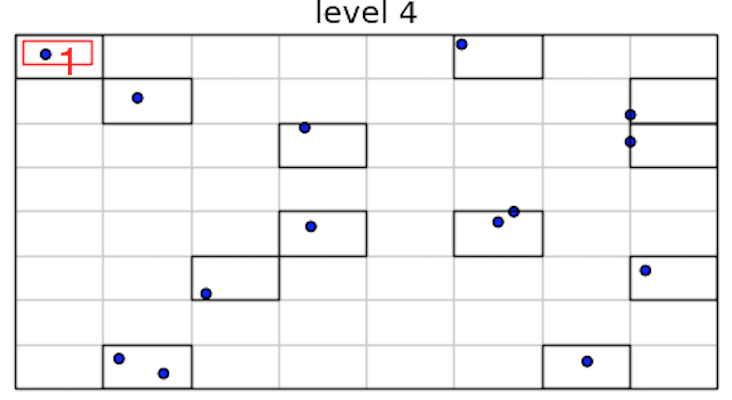
\includegraphics[width=\textwidth]{Images/1_1Quad1_4}
  \end{minipage}
  \hfill
  \begin{minipage}[b]{0.5\textwidth}
    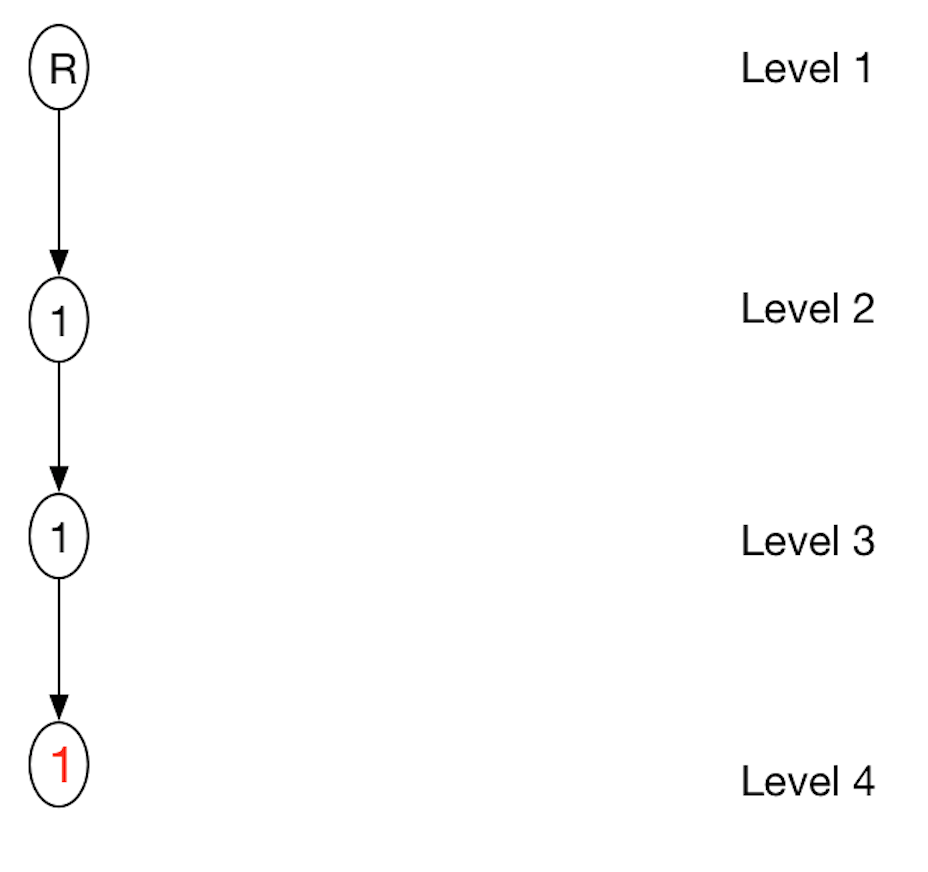
\includegraphics[width=\textwidth]{Images/1Quad_4_tree}
  \end{minipage}
  \vspace{0.5in}
  \caption{Sample Datapoints (left) and the Quadtree (right) at Level 4.}
  \label{fig:Level4}
\end{figure}

\subsubsection{Polygon overlapping 2 nodes}

Figure~\ref{fig:quad_1_1} shows the second scenario that demonstrates a condition where the query polygon overlaps 2 nodes at level 2 and the algorithm provides a medium performance. 

\begin{figure}[H]
  \centering
  \vspace{0.5in}
  \begin{minipage}[b]{0.35\textwidth}
    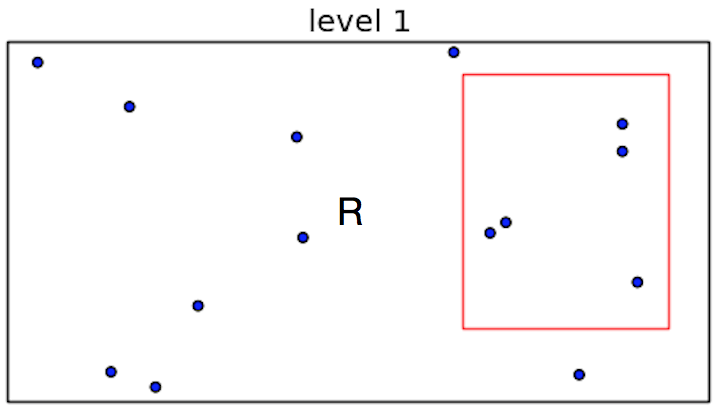
\includegraphics[width=\textwidth]{Images/2Quad_1}
  \end{minipage}
  \hfill
  \begin{minipage}[b]{0.6\textwidth}
    
\includegraphics[width=\textwidth]{Images/1_1Quad_1_tree}
  \end{minipage}
  \vspace{0.5in}
  \caption{Sample Datapoints (left) and the Quadtree (right) at Level 1.}
  \label{fig:quad_1_1}
\end{figure}

Figure~\ref{fig:quad_2_2} shows that at level 2, the algorithm isolates two quadrants (second and fourth child of the root node) and ignores the other two quadrants, thus bringing down the number of quadrants to be processed to 2.


\begin{figure}[H]
  \centering
  \vspace{0.5in}
  \begin{minipage}[b]{0.35\textwidth}
    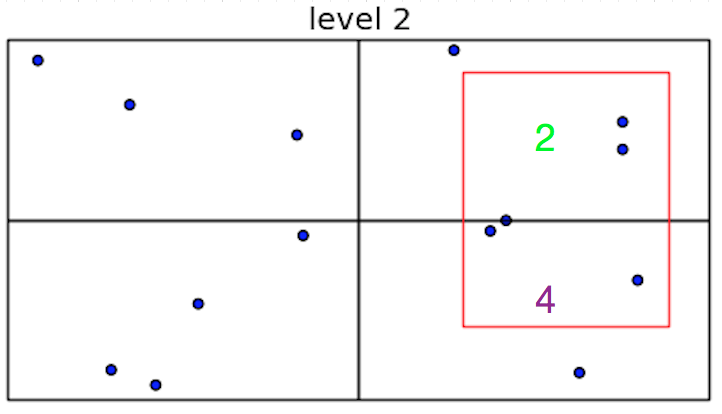
\includegraphics[width=\textwidth]{Images/2Quad_2}
  \end{minipage}
  \hfill
  \begin{minipage}[b]{0.6\textwidth}
    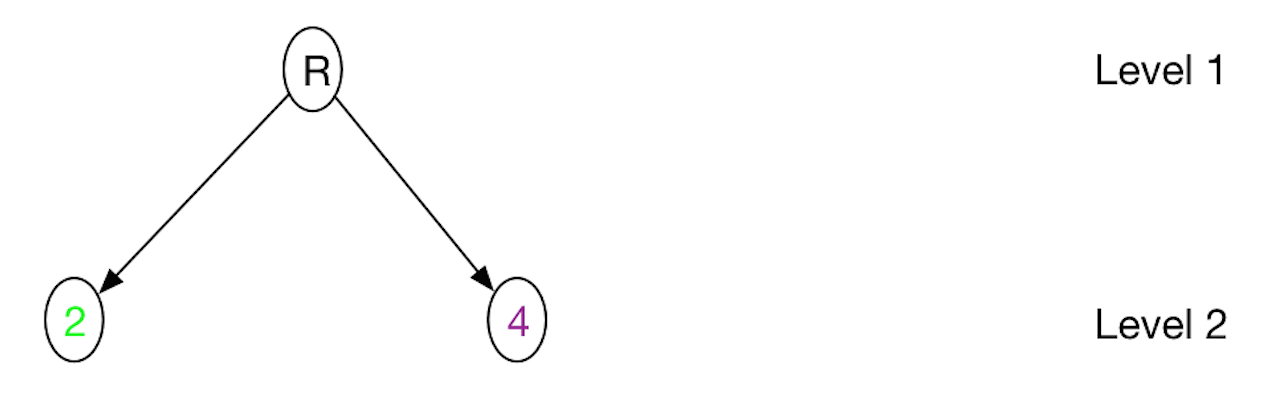
\includegraphics[width=\textwidth]{Images/2Quad_2_tree}
  \end{minipage}
  \vspace{0.5in}
  \caption{Sample Datapoints (left) and the Quadtree (right) at Level 2.}
   \label{fig:quad_2_2}
\end{figure}

Figure~\ref{fig:quad_2_3} shows that level 3, the algorithm isolates 7 quadrants which are the all four children of the second child of root node and first, second and fourth child of the fourth child of root node.
This step reduces the number of nodes to be processed by one as one of the child of the nodes output from the previous level is empty.

\begin{figure}[H]
  \centering
  \vspace{0.5in}
  \begin{minipage}[b]{0.35\textwidth}
    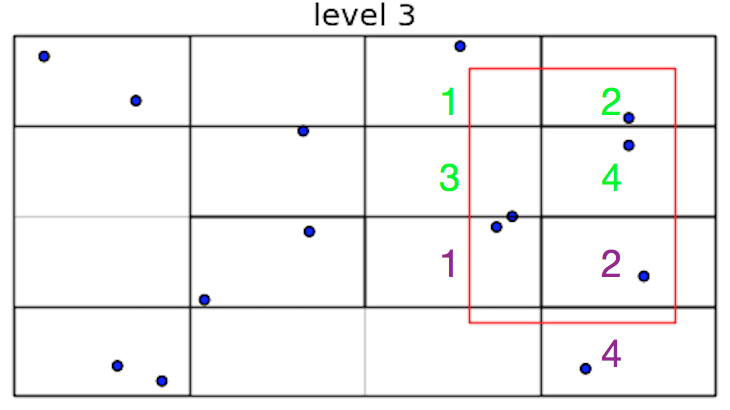
\includegraphics[width=\textwidth]{Images/2Quad_3}
  \end{minipage}
  \hfill
  \begin{minipage}[b]{0.6\textwidth}
    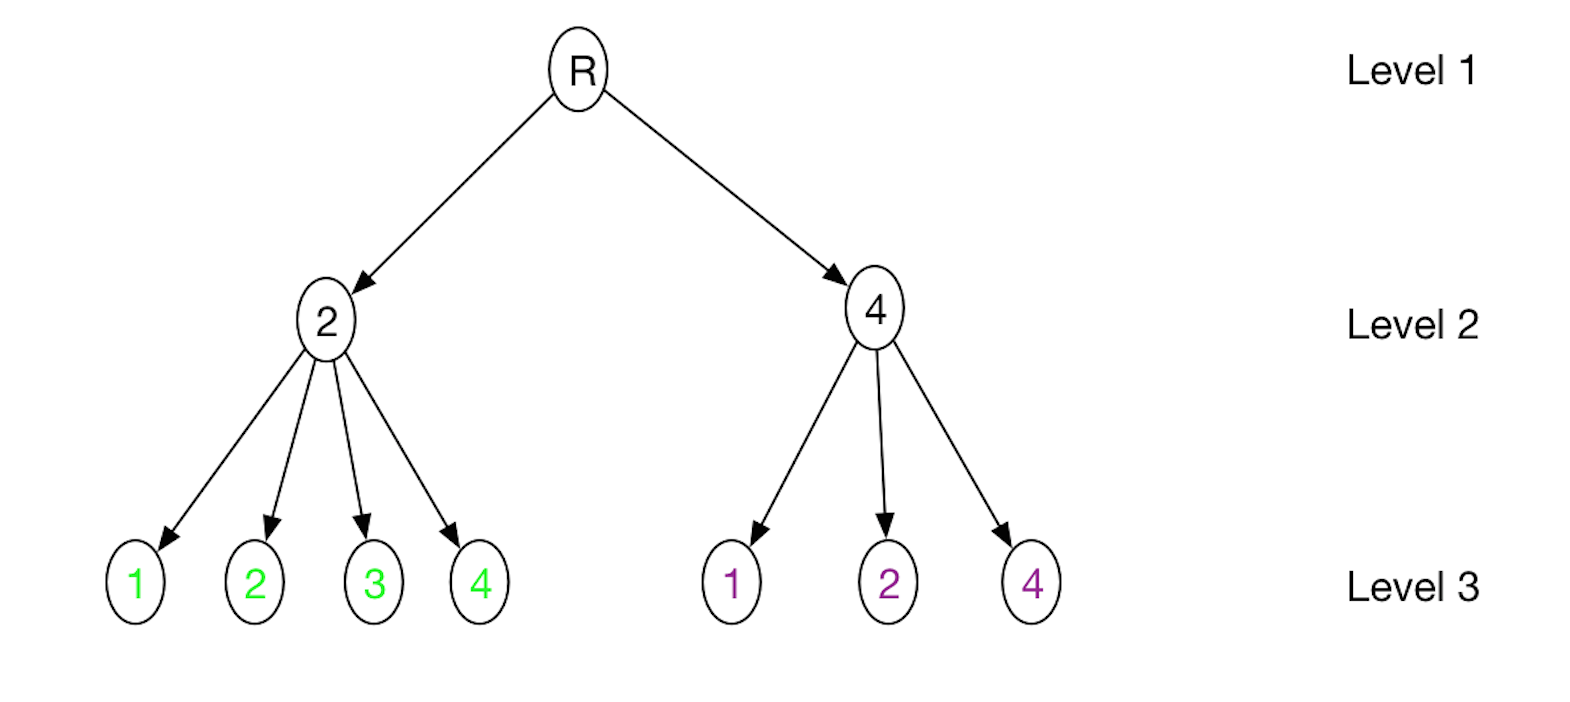
\includegraphics[width=\textwidth]{Images/2Quad_3_tree}
  \end{minipage}
  \vspace{0.5in}
  \caption{Sample Datapoints (left) and the Quadtree (right) at Level 3.}
  \label{fig:quad_2_3}
\end{figure}

Figure~\ref{fig:quad_2_4} shows that at level 4, the algorithm isolates 5 quadrants from the children of 7 quadrants from previous level. By traversing down to level 4, the number of data points that need to be evaluated are reduced by ignoring 3rd child of the 4th child from level 3. If the quadrant that is ignored at level 4 has a larger number of data points, then using a 3-level quadtree would have resulted in a huge performance penalty.
Finally only 5 quadrants at level 4 needs to be processed in order to get the points inside the polygon in this case.

\begin{figure}[H]
  \centering
  \vspace{0.5in}
  \begin{minipage}[b]{0.35\textwidth}
    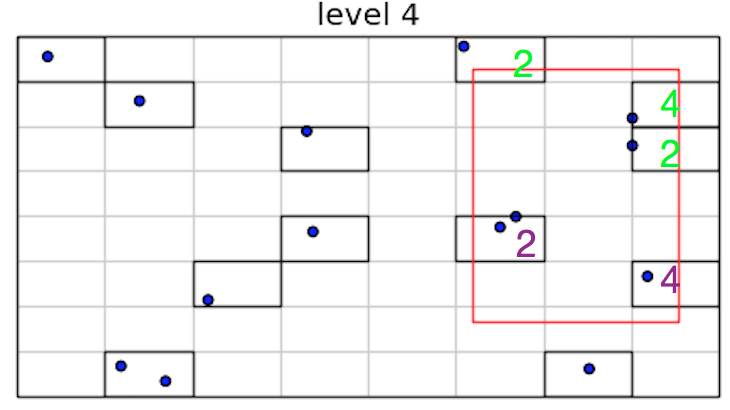
\includegraphics[width=\textwidth]{Images/2Quad_4}
  \end{minipage}
  \hfill
  \begin{minipage}[b]{0.6\textwidth}
    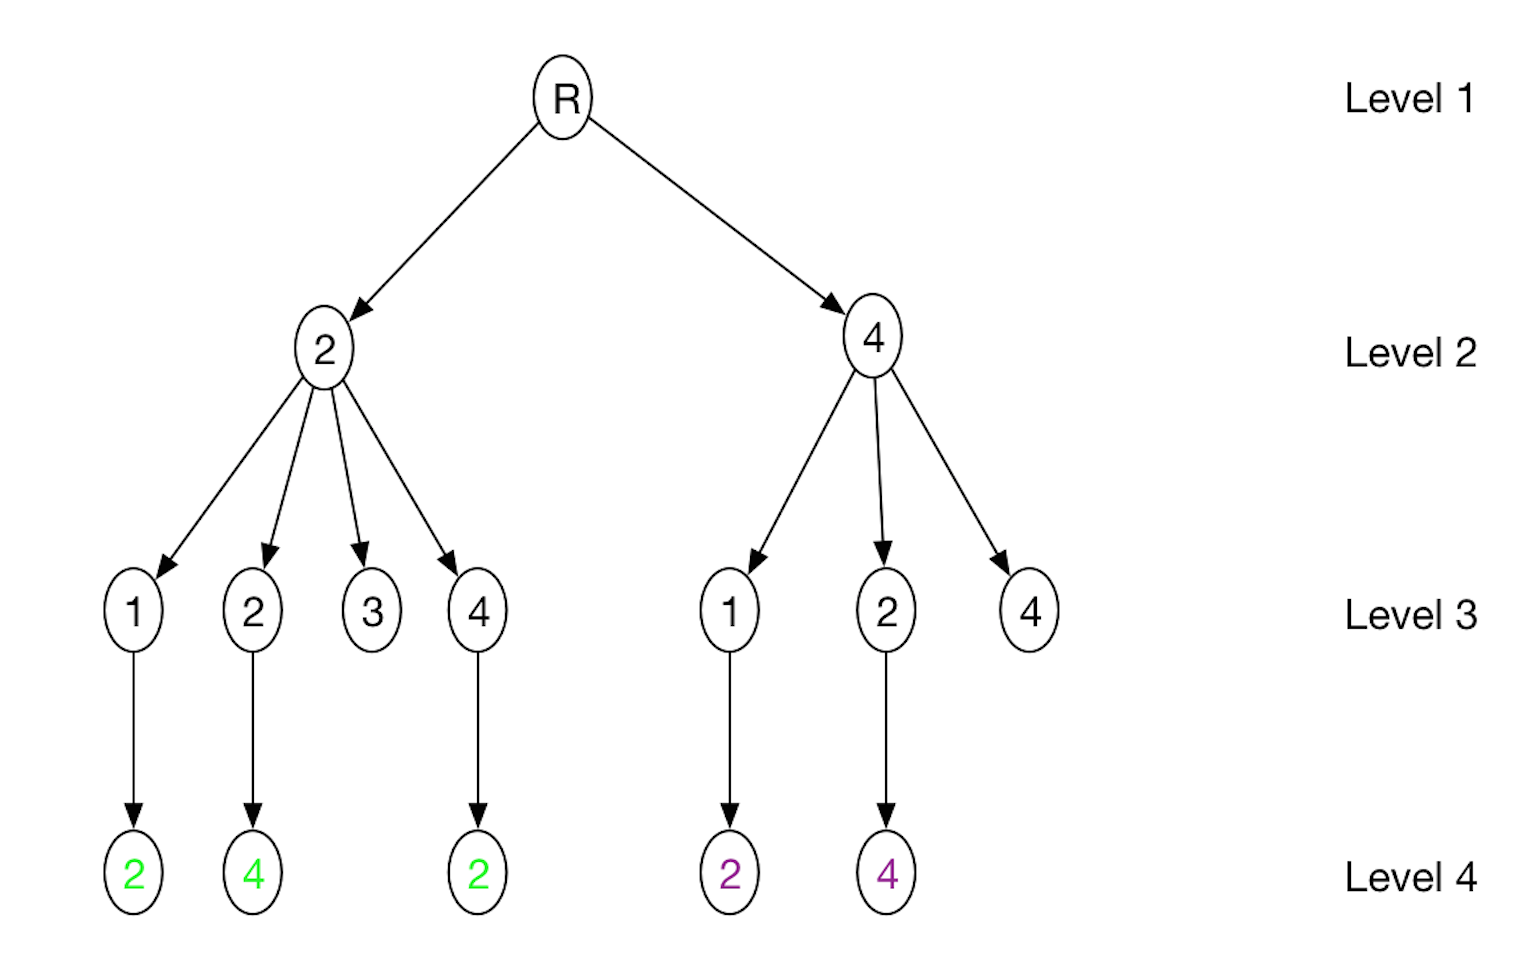
\includegraphics[width=\textwidth]{Images/2Quad_4_tree}
  \end{minipage}
  \vspace{0.5in}
  \caption{Sample Datapoints (left) and the Quadtree (right) at Level 4.}
  \label{fig:quad_2_4}
\end{figure}

\subsubsection{Query Polygon Overlapping all Leaf Nodes}

Figure~\ref{fig:quad_4_1} shows the last scenario that demonstrates a condition where the polygon contains maximum number of quadrants at level 4 of the quadtree and the algorithm provides least performance compared to all other scenarios.

\begin{figure}[H]
  \centering
  \vspace{0.5in}
  \begin{minipage}[b]{0.35\textwidth}
    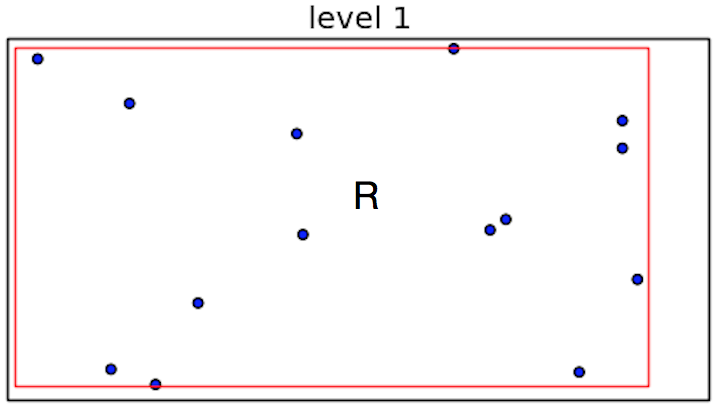
\includegraphics[width=\textwidth]{Images/4Quad1_1}
  \end{minipage}
  \hfill
  \begin{minipage}[b]{0.6\textwidth}
    
\includegraphics[width=\textwidth]{Images/1_1Quad_1_tree}
  \end{minipage}
  \vspace{0.5in}
  \caption{Sample Datapoints (left) and the Quadtree (right) at Level 1.}
  \label{fig:quad_4_1}
\end{figure}

In Figure~\ref{fig:quad_4_2} 
at level 2, the algorithm  overlaps all 4 quadrants at this level. Therefore the thread has to descend the tree from all four nodes.

\begin{figure}[H]
  \centering
  \vspace{0.5in}
  \begin{minipage}[b]{0.35\textwidth}
    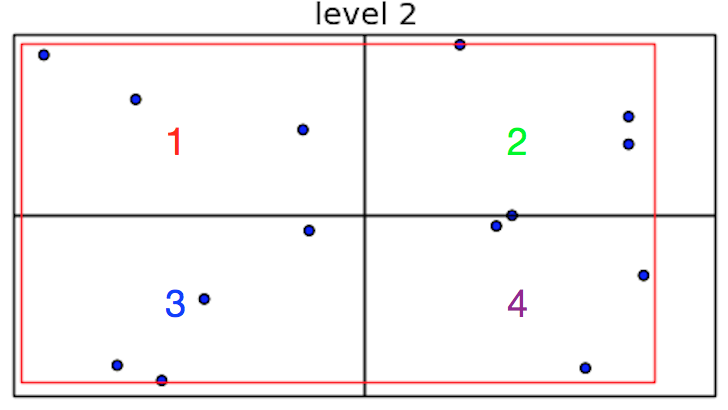
\includegraphics[width=\textwidth]{Images/4Quad1_2}
  \end{minipage}
  \hfill
  \begin{minipage}[b]{0.6\textwidth}
    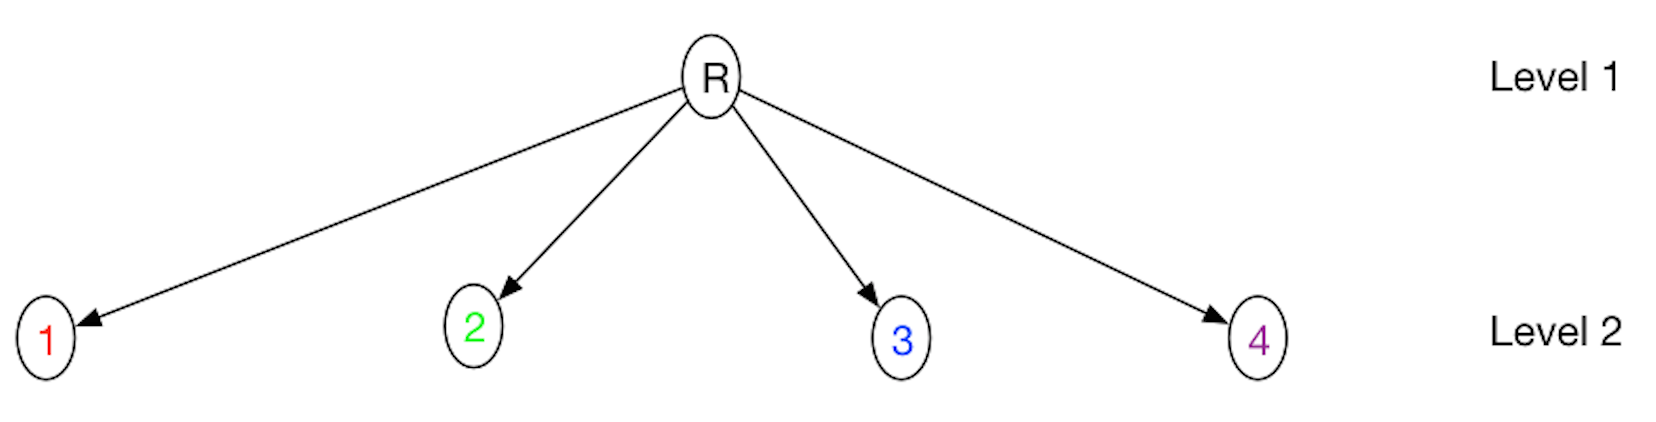
\includegraphics[width=\textwidth]{Images/1_1Quad_2_tree}
  \end{minipage}
  \vspace{0.5in}
  \caption{Sample Datapoints (left) and the Quadtree (right) at Level 2.}
  \label{fig:quad_4_2}
\end{figure}

In Figure~\ref{fig:quad_4_3} 
at level 3, the algorithm  isolates all 12 quadrants at this level. The maximum possible number of nodes at this level is 16 but four of  those nodes are empty nodes and these four nodes are ignored even though these nodes lie within the polygon.
\begin{figure}[H]
  \centering
  \vspace{0.5in}
  \begin{minipage}[b]{0.35\textwidth}
    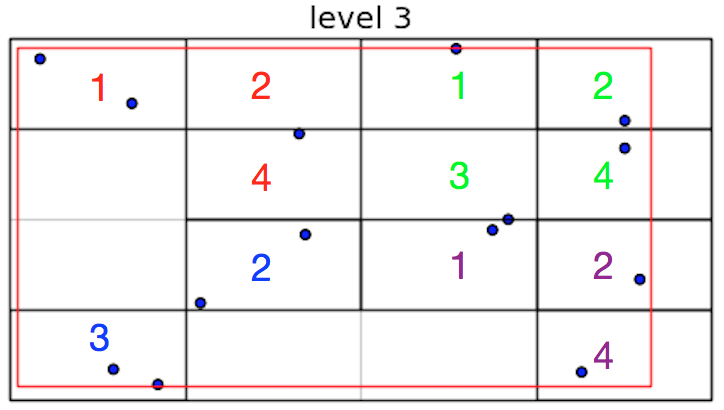
\includegraphics[width=\textwidth]{Images/4Quad1_3}
  \end{minipage}
  \hfill
  \begin{minipage}[b]{0.6\textwidth}
    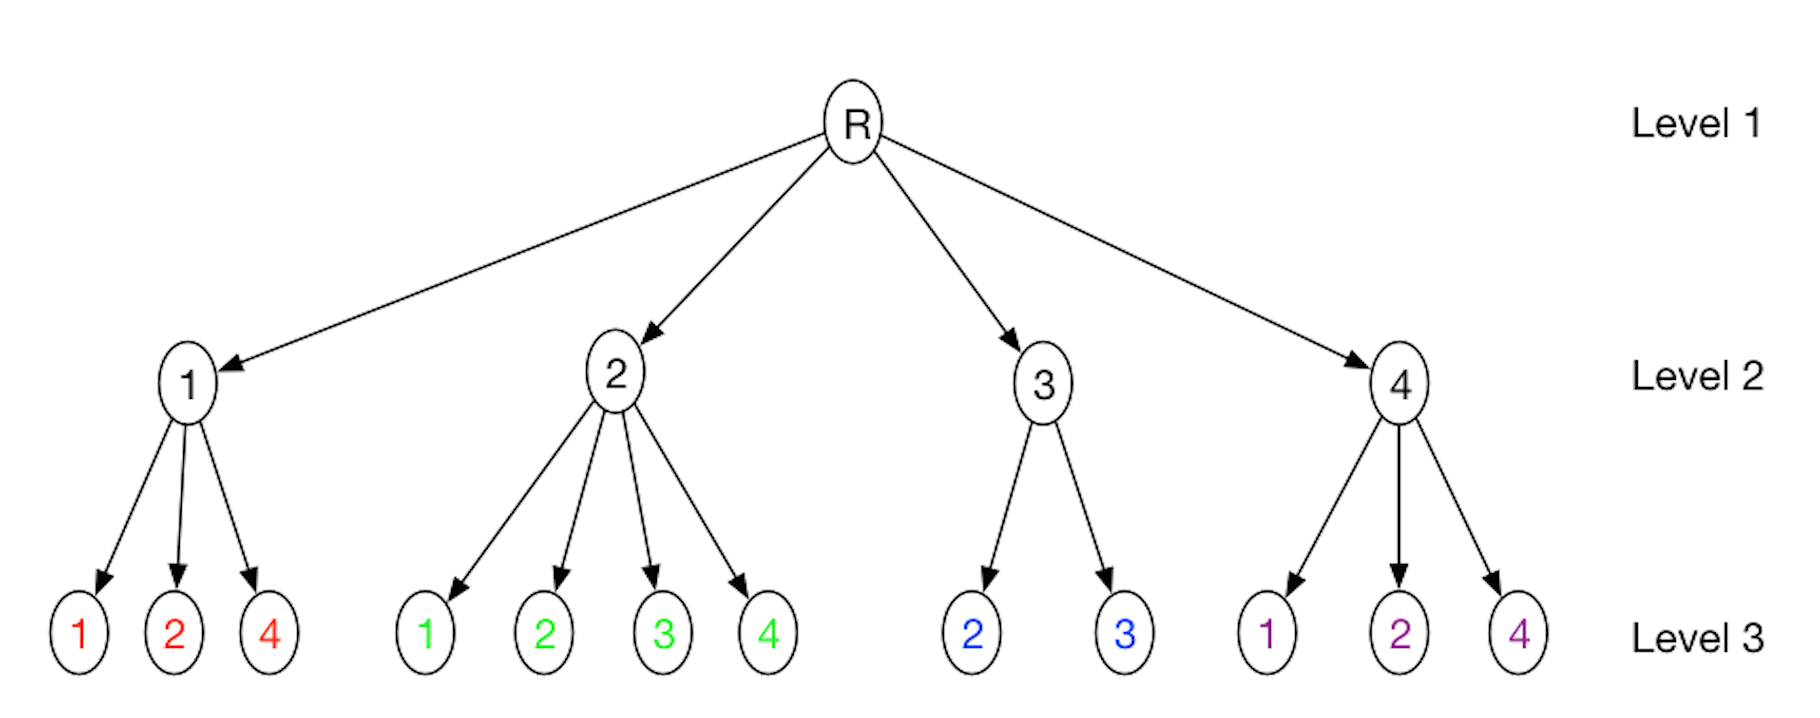
\includegraphics[width=\textwidth]{Images/1_1Quad_3_tree}
  \end{minipage}
  \vspace{0.5in}
  \caption{Sample Datapoints (left) and the Quadtree (right) at Level 3.}
  \label{fig:quad_4_3}
\end{figure}

Figure~\ref{fig:4Quad1_4} shows that at level 4, the algorithm isolates all the 12 quadrants at this level. The maximum possible number of nodes at this level is 64 but 52 of those nodes are empty nodes and  these 52 nodes are ignored even though these nodes lie within the polygon.
Finally only 12 quadrants at level 4 need to be processed in order to get the points inside the polygon in this case. If there are a larger number of data points distributed equally across the entire 2 D space and if there are no empty nodes, then all the 64 nodes need to be processed.

\begin{figure}[H]
  \centering
  \vspace{0.5in}
  \begin{minipage}[b]{0.35\textwidth}
    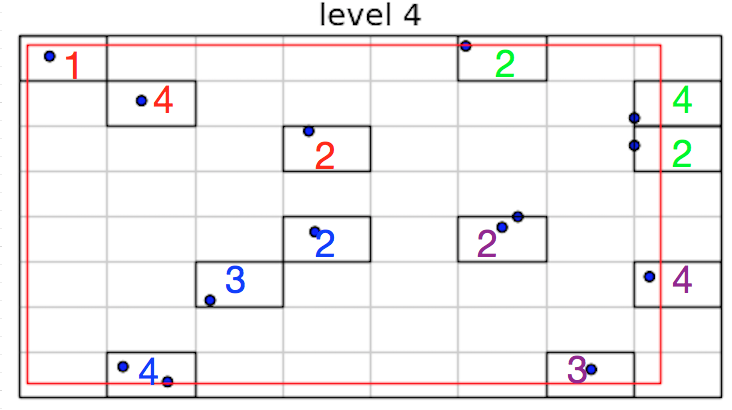
\includegraphics[width=\textwidth]{Images/4Quad1_4}
  \end{minipage}
  \hfill
  \begin{minipage}[b]{0.6\textwidth}
    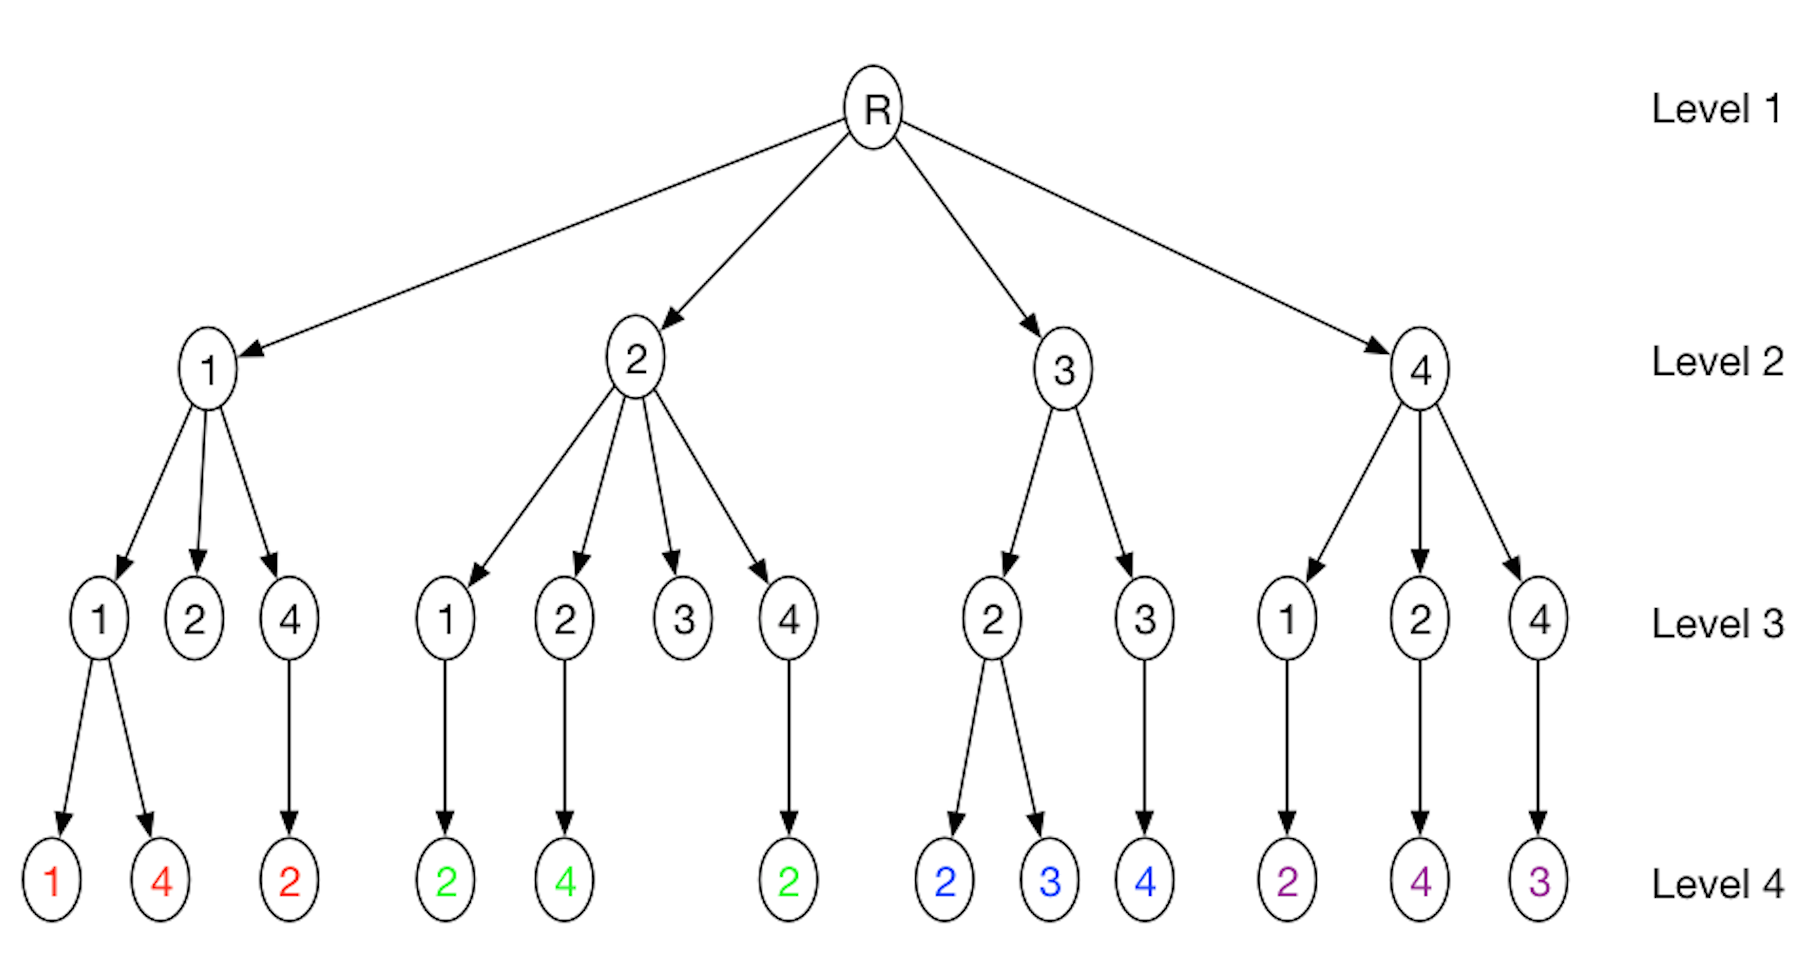
\includegraphics[width=\textwidth]{Images/1_1Quad_4_tree}
  \end{minipage}
  \vspace{0.5in}
  \caption{Sample Datapoints (left) and the Quadtree (right) at Level 4.}
  \label{fig:4Quad1_4}
\end{figure}

Figure~\ref{fig:Stack1}, shows the stack based iterative BFS traversal on GPU, in reference to Figure~\ref{fig:quad_4_3} 
and Figure~\ref{fig:4Quad1_4}. 

\begin{figure}[H]
\centering
\vspace{0.5in}
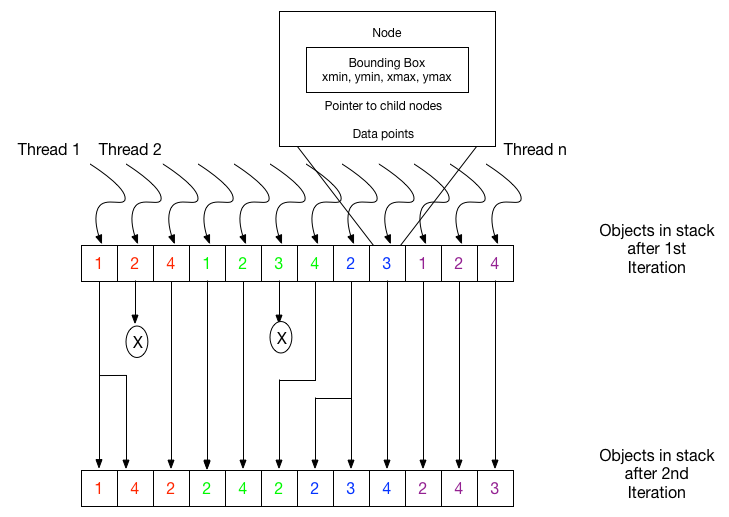
\includegraphics[scale=0.4]{Images/Stack1}
\vspace{0.5in}
\caption{Stack Based Iterative BFS Traversal.}
\label{fig:Stack1}
\end{figure}

\subsubsection{Query Polygon Containing no Points}

Figure~\ref{fig:1Quad_NoPoints} shows one case where the polygon overlaps a region where there are no points. 

\begin{figure}[ht]
  \centering
  \vspace{0.5in}
  \begin{minipage}[b]{0.35\textwidth}
    \includegraphics[width=\textwidth]{Images/NoPointQuad1}
  \end{minipage}
  \hfill
  \begin{minipage}[b]{0.6\textwidth}
    \includegraphics[width=\textwidth]{Images/1_1Quad_1_tree}
  \end{minipage}
  \vspace{0.5in}
  \caption{Sample Datapoints (left) and the Quadtree (right) at Level 1.}
  \label{fig:1Quad_NoPoints}
\end{figure}

Figure~\ref{fig:2Quad_NoPoints} shows two distinct cases. At level 2, the algorithm isolates first and third child of the root node.
At level 3, the polygon does not overlap with any of the children of the nodes from level 2. The nodes that it overlaps are empty nodes and therefore the tree is not traversed any further.

\begin{figure}[ht]
  \centering
  \vspace{0.5in}
  \begin{minipage}[b]{0.35\textwidth}
    \includegraphics[width=\textwidth]{Images/NoPointQuad2}
  \end{minipage}
  \hfill
  \begin{minipage}[b]{0.6\textwidth}
    \includegraphics[width=\textwidth]{Images/NoPoints3_1}
  \end{minipage}
  \vspace{0.5in}
  \caption{Sample Datapoints (left) and Quadtree (right) at Level 2.}
  \label{fig:2Quad_NoPoints}
\end{figure}




\chapter{Experimental Results}\label{chap:results}
%
% File - ch1.tex
%
%
% Description:
% This file should contain the first real chapter or section of your
% thesis.
%
%
The experimental results show that in many cases the GPU out-performs the CPU as
expected.  

\section{Results}
The performance is compared in terms of the number of polygons that can be queried per second. The number of polygons queried per second is measured for a wide range of input points. As the size of  data points increase, the performance of CPU diminishes at a faster rate than the GPU. In the case of GPUs, as the size of input increases, performance is affected as the amount of work done per thread increases and also the overhead of memory transfer of large amount of data between CPU and GPU increases.  But once the quadtree is transferred to the GPU, any number of polygons can be queried using iterative BFS traversal method described above.

Figure~\ref{fig:CPU_GPU_SmallPoly3}, Figure~\ref{fig:CPU_GPU_MediumPoly3} and Figure~\ref{fig:CPU_GPU_LargePoly3} show that the CPU-GPU approach gives a performance improvement 
by a factor of 3.2 for small datasets and a performance improvement by a factor of 449 for very large datasets in the case of small polygons, a performance improvement by a factor of 4 for small datasets and a performance improvement by a factor of 594 for very large datasets in the case of medium sized polygons and a performance improvement by a factor of 3.6 for small datasets and a performance improvement by a factor of 591 for very large datasets in the case of large sized polygons respectively.

\begin{figure}[H]
\centering
\vspace{0.5in}
\includegraphics[scale=0.5]{Images/CPU_GPU_SmallPoly3}
\vspace{0.5in}
\caption{Performance Comparison between CPU and GPU for Small Polygons.}
\label{fig:CPU_GPU_SmallPoly3}
\end{figure}

\begin{figure}[H]
\centering
\vspace{0.5in}
\includegraphics[scale=0.5]{Images/CPU_GPU_MediumPoly3}
\vspace{0.5in}
\caption{Performance Comparison between CPU and GPU for Medium Polygons.}
\label{fig:CPU_GPU_MediumPoly3}
\end{figure}

\begin{figure}[H]
\centering
\vspace{0.5in}
\includegraphics[scale=0.5]{Images/CPU_GPU_LargePoly3}
\vspace{0.5in}
\caption{Performance Comparison between CPU and GPU for Large Polygons.}
\label{fig:CPU_GPU_LargePoly3}
\end{figure}

The CPU performance diminishes at a faster rate than the GPU mainly because of the quadtree structure and the memory hierarchy. Since the tree is a pointer based structure, there is a cache miss every time a node is accessed. At the leaf node, the points are stored in a linked list, where each node in the list contains a pre-determined number of points and there is a cache miss every time a new buffer in the list is accessed. Therefore cache miss penalties are higher for larger datasets.

In the case of GPUs, the point buffers are sequentially stored in memory through memory preallocation. Though there is a penalty when a node is accessed, cache miss penalties are not encountered while reading data points from a node. And also, in the GPU implementation, the traversal is accelerated by starting the BFS at level 3 of the quadtree.

The Figure~\ref{fig:Different_Sized_Polygon_GPU4} shows the execution time of different polygon sizes on GPU. Similar to CPU, the GPU performs better on smaller polygons compared to the larger polygons.
In this case, the smaller polygons occupy 10 to 20 percent of the region  and the larger polygons occupy 70 to 90 percent of the region. Once the leaf nodes are reached, the number of nodes that need to be taken into account to compute points are very less  but for a large polygon which could contain a maximum of 64 nodes for a level 4 quadtree, points within all these 64 nodes need to be taken into account.

\begin{figure}[H]
\centering
\vspace{0.5in}
\includegraphics[scale=0.5]{Images/Different_Sized_Polygon_GPU4}
\vspace{0.5in}
\caption{Performance Comparison for Different Sized Polygons using GPU.}
\label{fig:Different_Sized_Polygon_GPU4}
\end{figure}

The performance is determined by the number of partial nodes a polygon contains because for partial nodes, each point inside a node needs to be checked against a polygon boundary whereas in the case of completely overlapping nodes only the range of points a node contains is stored.
The Figure~\ref{fig:LToMCmplxMedP} shows the execution time of individual medium sized polygons with a data input size of 3000. The polygons are ranked based on the number of partial nodes it contains and its execution time is measured. As the number of partial nodes increase, the execution time per polygon increases.
The number of polygons calculated per second is the average of the output of all these individual polygons.

\begin{figure}[H]
\centering
\vspace{0.5in}
\includegraphics[scale=0.5]{Images/LToMCmplxMedP}
\vspace{0.5in}
\caption{Execution Time of Least to Most Complex Medium Sized Polygons.}
\label{fig:LToMCmplxMedP}
\end{figure}

Figure~\ref{fig:SpeedUp} shows the performance comparison between CPU and GPU measured for different sizes of polygons. The significant speed up on GPU is due to the memory coalesced access and due to accelerating the traversal by starting the BFS from level 3. In this case, the algorithm traverses one level down the tree to quickly find the set of nodes that satisfy the query, 

The maximum performance gain is achieved for the medium polygons which are more computationally intensive than small polygons. Very less number of threads are active for small polygons and this does not take advantage of the throughput oriented nature of the GPU. The work on medium sized polygons is optimum for the GPU as the performance decreases a little for larger polygons. The performance is mainly determined by the number of partial nodes a polygon contains. In the case of CPU, all the partial nodes in a polygon are processed sequentially but in the case of GPU, 32 partial nodes within a polygon are computed in parallel with 48 (Total number of SMX x (CUDA cores per SMX / number of polygons per warp))~\cite{nvidia:12:gtx680tech} polygons being computed simultaneously.

\begin{figure}[H]
\centering
\vspace{0.5in}
\includegraphics[scale=0.5]{Images/SpeedUp}
\vspace{0.5in}
\caption{Speed Up of GPU over CPU.}
\label{fig:SpeedUp}
\end{figure}



\chapter{Conclusion}\label{chap:conclusion}

%%%%%%%%%%%%%%%%%%%%%%%%%%%%%%%%%%%%%%%%%%%%%%%%%%%%%%%%%%%%%%%%%%%%%%%%%%%%%%%
The range search which is a fundamental operation in GIS and spatial databases always performs better when a spatial data structure is used and its performance is further improved when the search is implemented on a GPU.
This paper has proved that an irregular pointer based quadtree  need not be linearized in order to achieve a significant performance gain on GPU. And the CPU-GPU approach provides a speed up of 3x to 500x than the pure CPU approach. 
In a real world scenario, the range search problem is carried out on irregular polygons. For future work,  the work presented in this paper can be extended to implement PIP search on irregular polygons. 
The work on the GPU can be extended to compute larger data sets as the size of RAM per GPU increases. With increase in shared memory size, quadtrees with deeper layers can be traversed. There would be a significant improvement in the performance with increase in shared memory size and increase in global memory bandwidth.









%%%%%%%%%%%%%%%%%%%%%
% Back-matter
%%%%%%%%%%%%%%%%%%%%%

%%%%%%%%%%%%%%%%%%%%%%%%%%%%%
% For the bibliography there are two options. (1) You can create a  master file
% called thesis.bib (template included in this % collection of files) and use
% the \bibliography{thesis}  command. The advantage is that thesis.bib can be
% used for other papers (2) You can create the file thesis_bib.tex which is a
% list of references specifically for this thesis.
%%%%%%%%%%%%%%%%%%%%%%%%%%%%%

%%%%%%%%%%%%%%%%% Option 1 %%%%%%%%%%%%%%%%%%%%%%
%\nocite{*} % forces all references to be printed.

\bibliographystyle{plain}
\bibliography{thesis}

%%%%%%%%%%%%%%%%%%%%%
% Appendices
%%%%%%%%%%%%%%%%%%%%%
\begin{appendix}
\chapter{CUDA Code for Brute Force Search} \label{appendix1}
%
% File - appendix1.tex
%
%
% Description:
% This file should contain your first set of appendix material.
%
%
%
\lstinputlisting{bruteforce.c}
\chapter{Header File for Memory Allocation} \label{appendix2}
\renewcommand{\theequation}{B.\arabic{equation}}
%
% File - appendix2.tex
%
%
% Description:
% This file should contain your second set of appendix material.
%
%
%
\lstinputlisting{MemoryManager.h}

\chapter{CUDA C Code for PIP Search on GPU} \label{appendix3}
\renewcommand{\theequation}{B.\arabic{equation}}
%
% File - appendix2.tex
%
%
% Description:
% This file should contain your second set of appendix material.
%
%
%
\lstinputlisting{cdpQuadtree.cu}

\end{appendix}

%%%%%%%%%%%%%%%% Option 2 %%%%%%%%%%%%%%%%%%%%%%%%%%
%\input thesis_bib.tex
\end{document}
